\documentclass[11pt]{book}
\usepackage{graphicx}
\usepackage[margin=1in,bindingoffset=.2in]{geometry}
\usepackage[backend=biber, style=ieee]{biblatex}
\addbibresource{references.bib}
\usepackage[parfill]{parskip}
\usepackage{courier,textcomp,amsmath,listings, color}
\usepackage{float}
\newcommand{\code}[1]{\texttt{#1}}
\usepackage{longtable}
\usepackage{tcolorbox}
\usepackage[titletoc]{appendix}

% CODE HIGHLIGHTING COLOURS SET UP
% Set up for C#, Credit: http://tex.stackexchange.com/questions/124953/syntax-highlighting-in-listings-for-c-that-it-looks-like-in-visual-studio
%\setmonofont{Consolas} %to be used with XeLaTeX or LuaLaTeX
\definecolor{bluekeywords}{rgb}{0,0,1}
\definecolor{greencomments}{rgb}{0,0.5,0}
\definecolor{redstrings}{rgb}{0.64,0.08,0.08}
\definecolor{xmlcomments}{rgb}{0.5,0.5,0.5}
\definecolor{types}{rgb}{0.17,0.57,0.68}

\lstset
{
  language=Ruby,
  captionpos=b,
  %numbers=left,
  %numberstyle=\tiny,
  frame=lines,
  showspaces=false,
  showtabs=false,
  breaklines=true,
  showstringspaces=false,
  breakatwhitespace=true,
  escapeinside={(*@}{@*)},
  commentstyle=\color{greencomments},
  morekeywords={partial, var, value, get, set},
  keywordstyle=\color{bluekeywords},
  stringstyle=\color{redstrings},
  basicstyle=\ttfamily\small,
}

\begin{document}
\begin{titlepage}
	\newgeometry{margin=1in}
	\begin{center}
		{\huge Advanced Querying and Analysis\\ of Git Repositories\\}
		\vspace{1.5cm}
		{\Large \textbf{Daniel Brown} \\}
		{\Large Department of Computer Science, University of York \\}
		\vspace{1.5cm}
		
\includegraphics[width=100px]{images/university-of-york-shield} \\
		\vspace{1.5cm}
		{\Large September 2015 \\}
		\vspace{1.5cm}
		\Large Supervised by Dr. Dimitris Kolovos \\
		\vspace{1.5cm}
		\Large A thesis submitted in partial fulfilment for the degree of \\ \textit{Master of Science in Advanced Computer Science}\\
		\vspace{5cm}
		\small 9,983 words as counted by Texpad.app
	\end{center}
	\restoregeometry
\end{titlepage}

\chapter*{\centering Abstract}
\addcontentsline{toc}{chapter}{Abstract}
\begin{center}
	\parbox{350pt}{
Git is one of the most popular version control systems available \cite{gitpopularity} and, as well as many privately hosted instances, powers the well-known social programming website GitHub \cite{gitpowersgithub}.

Despite Gits popularity there are few systems available for analysing a git repository or querying it for useful metrics such as most popular commit time, largest commit, most active contributor or something more complex.

The systems that do exist to analyse Git repositories, namely GitInspector \cite{gitinspector} and Github, don't allow for custom queries to be written by the user. Meaning, for example, you cannot ask the question "What day of the week is Daniel most likely to author a commit of over 100 lines" or "Which contributor has had the highest percentage of their committed lines changed by someone else". 

This project presents a tool, called EpsilonGit, which allow users to write these custom queries by letting them interact with a git object database as a model using the Epsilon platform and its associated domain specific modelling languages. This model-based solution is then compared with existing technologies on the parameters of code complexity, speed, and extensibility by the user.
}
\end{center}

\clearpage

\section*{Acknowledgement}
I would like to take this opportunity to thank Dr. Dimitris Kolovos who not only provided support and encouragement throughout the course of this project, but also came up with the original idea of using model driven engineering to interact with git and added features into the Epsilon suite to support some of the work I was doing.

A special thank-you is extended to my parents, siblings and girlfriend who have supported me throughout the trials and tribulations of my time at York by visiting both myself and the National Railway Museum an inordinate amount of times. The same gratitude is required of my friends both from at home in Dunstable and The University of Hull, where I completed my Bachelors degree. %The museum bit is an inside joke. I'll keep it in for a laugh

\section*{Statement of Ethics}
Ethics in research is of paramount importance and therefore this project has been carried out with them in mind at every step. 

All literature, ideas and code that has been used in the formation of this project has been correctly referenced and credit has been given where it is due.

The data that my project interacts with is a local copy of a git database. The user must source this data on their own, and therefore the project doesn't have to deal with any authentication or security. EpsilonGit only gives people a different view on data they already have.

No other significant ethical issues related to this project could be identified.

\tableofcontents

\listoffigures
 
\listoftables

\chapter{Introduction}
\label{introandbackground}
\section{Introduction and Background}
% Rough outline of git 
	% (e.g. its a distributed VCS... so people have code locally to be modelled, people use it for x functions (e.g. commit, branch, put their name to code) )
	% Why would someone what to query and analyse their git repository?
	% Some cool questions that could be asked
	
Git is a free and open source distributed version control system \cite{gitintro} that is designed to allow users to manage changes to files, often source files in a software project. This enables developers to "roll back" to a previous version of a file, see the difference between a file at two different times or determine which team member authored a line of code. 

Version control best practices suggest that a developer should be committing code a little at a time and quite often \cite{gitbestpractices}, this makes it a good place to analyse to determine an individual developer or teams working practices in retrospect.

A project manager may want to analyse a git repository to answer questions such as "How large is the average commit size?", "What time of the day are most commits made?" and "Which of my developers is committing the most code that is later replaced?". The answers to these questions may allow improvements in both quality of code and workplace practices.

Mining Software Repositories (MSR) for information to improve Software Engineering practices is a hot area of research right now with an annual dedicated conference \cite{msr2015}. MSR is the process of analysing the rich data available in these repositories to uncover interesting and actionable information about software systems \cite{theroadagainformsr} including identifying pre-existing patterns in code, and automatically linking code to bug reports -- this project aims to aid that discovery. Answering semantically challenging questions such as "Does the git fork flow enable more people to contribute to this project?" could be achieved, potentially changing the shape and attitudes of organisations.

Whilst MSR is a popular research topic a recent paper enumerating the tools used by MSR researchers found that many MSR researchers are using general purpose data mining tools rather than bespoke specialised MSR tools \cite{toolsinminingsoftwarerepositories}.

% Rough outline of modelling
	% What is modelling?
	% Why is it _possibly_ suitable for this project?
Model Driven Engineering is an approach to tackle the complexity of data, and how it is interacted with, through the use of high level abstractions called models \cite{modeldrivenengineering} and a set of Domain-specific modelling languages and Transformation engines and generators.   
	
Due to the large array of features provided by git and the widespread use of hashes and graph data structures in the underlying system it is often considered to be complex \cite{gitcomplex}\cite{githard}\cite{gitmixedmetaphors}.

The proposition of this project is that a model driven engineering solution to querying and analysing git repositories can deliver substantial productivity and quality improvements over existing approaches as it removes much of the complexity associated with git.

% Discussion of epsilon
% Discussion of the epsilon driver framework and what integrating with epsilon gets us (e.g. ability to make HTML from models, use of EOL Language, ability to run in and out of eclipse, etc)

Epsilon is a family of languages and tools for code generation, model-to-model transformation, model validation, comparison, migration and refactoring \cite{epsilonhomepage}. Whilst Epsilon comes with support for interacting with EMF, XML and several other types of model formats out-of-the-box it also has a system called the Epsilon Model Connectivity layer which allows developers to implement drivers for other types of models and structured artefacts.

Epsilon was originally developed with a focus on software engineering models (e.g. UML models), due to its modularity and extensibility it has also been used on non-model artefacts such as spreadsheets, XML documents and relational data. This project aims to bring git access capabilities to the Epsilon Platform.

The project being introduced here, EpsilonGit, will be deemed a success if it displays the following characteristics: is as fast, or faster, as competing solutions for identical queries; allows users to write custom queries in more concise and less complex code than interacting with git directly, and has coverage of the most common parts of gits features.

\section{Motivation}
% Motivation
	% Improve companies, open source projects and individuals understanding of their code and workflows
	% Encourage people to use and invest in Modelling, particularly using epsilon
	% Release it to the world and see what innovative and cool information people could get from their git repositories. With open data and software all kinds of weird shit can be done the original creator wouldn't have thought of.
The Joel Test \cite{joeltest} is often cited as a simple list of best practices for software development. Rule number 1 is to use version control software in order to aid teamwork, maintain a canonical history of source code and reduce the likelihood of losing any work. The positive impact that version control has means that many open source, individual and commercial projects use version control -- one of the most popular being git \cite{gitpopularity}. 

Although many projects use git there are very few tools for querying and analysing the metadata and other information contained within git repositories. Those that are available lack the ability to add user-designed custom queries. 

The reasons that there are few good tools for querying git repositories are varied. Firstly, Mining Software Repositories is a relatively new field --  meaning both that no one has built these tools yet and the Software Engineering community at large doesn't know of the benefits. Secondly the git API isn't the easiest to work with. Understanding the git command line requires knowledge of many Unix commands and is just one of the reasons Git is often said to be complicated \cite{gitcomplex}\cite{githard}\cite{gitmixedmetaphors}. Listing \ref{lst:gitbash} shows that to list authors by number of commits you need to have knowledge of Bash, Awk, Sort, Cut and Git itself.\\ 

\begin{lstlisting}[caption=List Authors by Number of Commits in Git Bash, label=lst:gitbash]
git log --format='\%aN <\%aE>' | awk '{arr[\$0]++} END{for (i in arr){print arr[i], i;}}' | sort -rn | cut -d\ -f2-
\end{lstlisting}

Through developing a system in which users can write their own custom queries in an easy-to-use and abstract fashion it is anticipated that teams will be able to learn more about their own workflows and where improvements can be made -- this could be particularly useful to teams using agile methodologies which lack the rigid structure of older methods such as Waterfall.

The software produced as part of this project should also make it easier to determine if git best practices \cite{gitbestpractices} are being followed. In addition to best practices some teams set project wide best practices for commit messages \cite{erlanggitcommitmessages}, users should be able to write validators to ensure these are being used.

As well as helping teams understand their git repositories this project also aims to encourage Software Engineers to learn about and invest in Model-Driven Engineering. It is the the hope of the author that combining MDE with a technology as prevalent as git may help to widen its appeal. In particular it would be great if this attracted more people to the open source Epsilon MDE platform \cite{epsilonhomepage}.

One of the more interesting aspects of the project will be opening up a world of newly accessible data to people and seeing what interesting analysis they can come up with that the author alone wouldn't have thought of.

\section{Aims and Objectives}
\label{aimsandobjectives} 
%Aims and objectives
	% Develop a solution which covers all of the most common parts of git (e.g. Object Model, Branches, Authors and Committers)
	% Develop a solution which has as fast or faster runtime for the same output as GitInspector / Github / GitSQL
	% Develop a solution which requires less code, and code of lower complexity for the same output as other solutions
	% Develop a solution which, at the same times, provides high level simple nice clean interaction whilst allowing access to low level stuff for those who also want that interaction
This project aims to implement an Epsilon Model Connectivity (EMC) driver to enable querying and analysis of git repositories from the domain-specific programming languages of the Epsilon Eclipse framework.

The objectives of the project are as follows:

\begin{enumerate}
	\item Develop a EMC solution for interacting with the most commons parts of Git (Object Model, Branches and Author \& Committer Information) through Epsilon Eclipse
	\item Optimise the solution so that it produces the same output as GitInspector in the same amount of time or less 
	\item The solution should allow developers to write queries with identical output to GitInspector and GitHub with less code, and code of less compexity
	\item The solution should provide access to all low-level properties of the covered areas of git whilst providing higher-level methods to speed up development of user-written queries
\end{enumerate}

A secondary aim of the project is to attract more users to the Epsilon Platform and model driven engineering in general using git prevalence in Software Engineering as a draw.

\section{Constraints}
\label{constaints}
There are several constraints which could have an effect on the outcome of this project. 

\begin{enumerate}
	\item This project is to be completed in the 4 months between the end of the taught portion of a Masters degree and the following September. In that time the author also has to interview for opportunities of employment so even less time can be allocated to EpsilonGit.
	\item This project is also the first full-fledged academic paper of the author and therefore his knowledge of this area is limited
\end{enumerate}

The author hopes to overcome these issues to provide a valid and novel piece of research.

\section{Report Structure}
% Report Structure
	% A paragraph or two explaining the overall flow of this document, and calling out the names of each chapter. Not repeating the table of contents, but instead highlighting important sections in prose.

This paper covers the entire process of development of EpsilonGit.

Chapter 2 covers a literature review undertaken before work was carried out, model driven engineering and the git object model are discussed in detail. Using the information ascertained in the literature review chapter 3 discusses the requirements of this project. Chapter 4 discusses several software engineering methodologies that could be followed during the course of development and a decision is made.

Chapter 5 explains the processes undertaken during the design stage, including the interaction between JGit and the Epsilon Model Connectivity layer. The actual implementation details of EpsilonGit are discussed at length in Chapter 6. Chapter 7 rounds up the practical portion of the report by explaining how several types of testing were used together to form a complete testing framework for the EMC driver.

Chapter 8 evaluates the work undertaken against the aims and objectives which were set out in section \ref{aimsandobjectives}. Conclusions from the work are drawn in Chapter 9 and potential future work ideas are provided to the reader. Finally, Chapter 10 reflects on the project as a whole and the author himself.  

\chapter{Literature Review}
% Intro paragraph "This chapter looks at the existing literature... etc"
% Section on literature about Git and the git object model
	% Conclusions drawn from the literature
		% A well known model, with some interesting idiosyncacies. Fits modelling well.
		
\label{litreview}
This chapter looks at the existing literature in the relation to the Git Object Model, Model Driven Engineering techniques, Previous attempts at analysing git repositories and techniques for interacting with object models -- such as the HTML Document Object Model -- which are similar to Git.

\section{Git and Version Control Systems}
\label{sec:git}
Version control systems (VCS) allow Software Engineers to keep a history of changes made to the files they work with. Diomidis Spinellis of Athens University of Economics and Business states that adopting a VCS can be the most important tooling improvement a Software Engineering team can make \cite{toolsofthetrade}.

Git is a version control system originally developed by Linus Torvalds, known for developing the Linux Kernel, with the goals of being fast and efficient with large projects \cite{progit}.

There are two main types of VCS, Centralised Version Control Software and Distributed Version Control Software. Centralised version control systems rely on a central server which contains the canonical source repository whilst distributed systems downloads a complete clone of the repository with a full commit history, meaning each client has a first class repository\cite{whydistributed}.

Distributed version control software has several advantages over centralised systems. Firstly they allow any developer to have write access to a repository, rather than having to submit a patch to someone with committer privileges, which lowers the barrier to entry on open source projects \cite{distributedimpactoss}. Secondly they allow cheap local branching and merging as well as reduced redundant file storage thanks to the use of changesets rather than individual file revisions \cite{distributedimpactoss}. 

Whilst distributed version control systems \cite{whydistributed}, and in particular git \cite{gitpopularity}, have become more popular than centralised version systems there are still some proponents of CVS thanks to the fact that engineers don't have to download potentially very large repositories with very large histories \cite{cvsvsvcs}.

Git uses the distributed model, meaning each computer on which a repository is used has a complete copy of its history. This makes it a good candidate for analysis as any team member will be able to be involved in the process rather than just the central repository administrator.

Although there are many methodologies for using version control systems all of them contain the same basic commands which form the majority of a users interaction with their VCS. In Git these commands are \cite{gitrefbasic}: 

\begin{table}[h]
\centering
\begin{tabular}{| l | p{9cm} |}
\hline
\textbf{Command} & \textbf{Action} \\ \hline
git clone [remote repository location] & Downloads a repository and all its history from a specified remote location \\ \hline
git add [file] & Adds a file to the git index so that its changes will be tracked \\ \hline
git commit [message] & Stores current changes to history with a message to inform other engineers why changes were made \\ \hline
git push & Sends local changes to a remote repository \\ \hline
\end{tabular}
\caption{Basic Git Commmands}
\label{tab:basic-git-commands}
\end{table}

The git community has developed several different workflows to interact with git for different types of projects and requirements of those projects \cite{gitcomparingworkflows}. 4 such examples are: 

\begin{enumerate}
	\item Centralized Workflow; which works in much the same way as a CVS would
	\item Feature Branch workflow which requires engineers to create a new branch for each feature they are working on before merging back into a main branch which is considered the production ready code
	\item The Gitflow Workflow; which is a mixture of the two previous workflows
	\item Forking Workflow; Commonly used by open source projects. A contributor makes changes in his own local repository and then requests that they be 'pulled' into the main public repository
\end{enumerate}

The many different ways of using git suggest that different analytics may also be required.

\clearpage

\section{The Git Object Model}
\label{gitobjectmodel}
The core of git is a content-addressable filesystem which can store any object and assign it a hashcode by which it can be identified \cite{progit}. There are 4 main types of object stored in this system, known as the git object model, which are shown in Figure \ref{fig:gitobjectmodeldiagram}.

\begin{figure}[h]
	\centering
	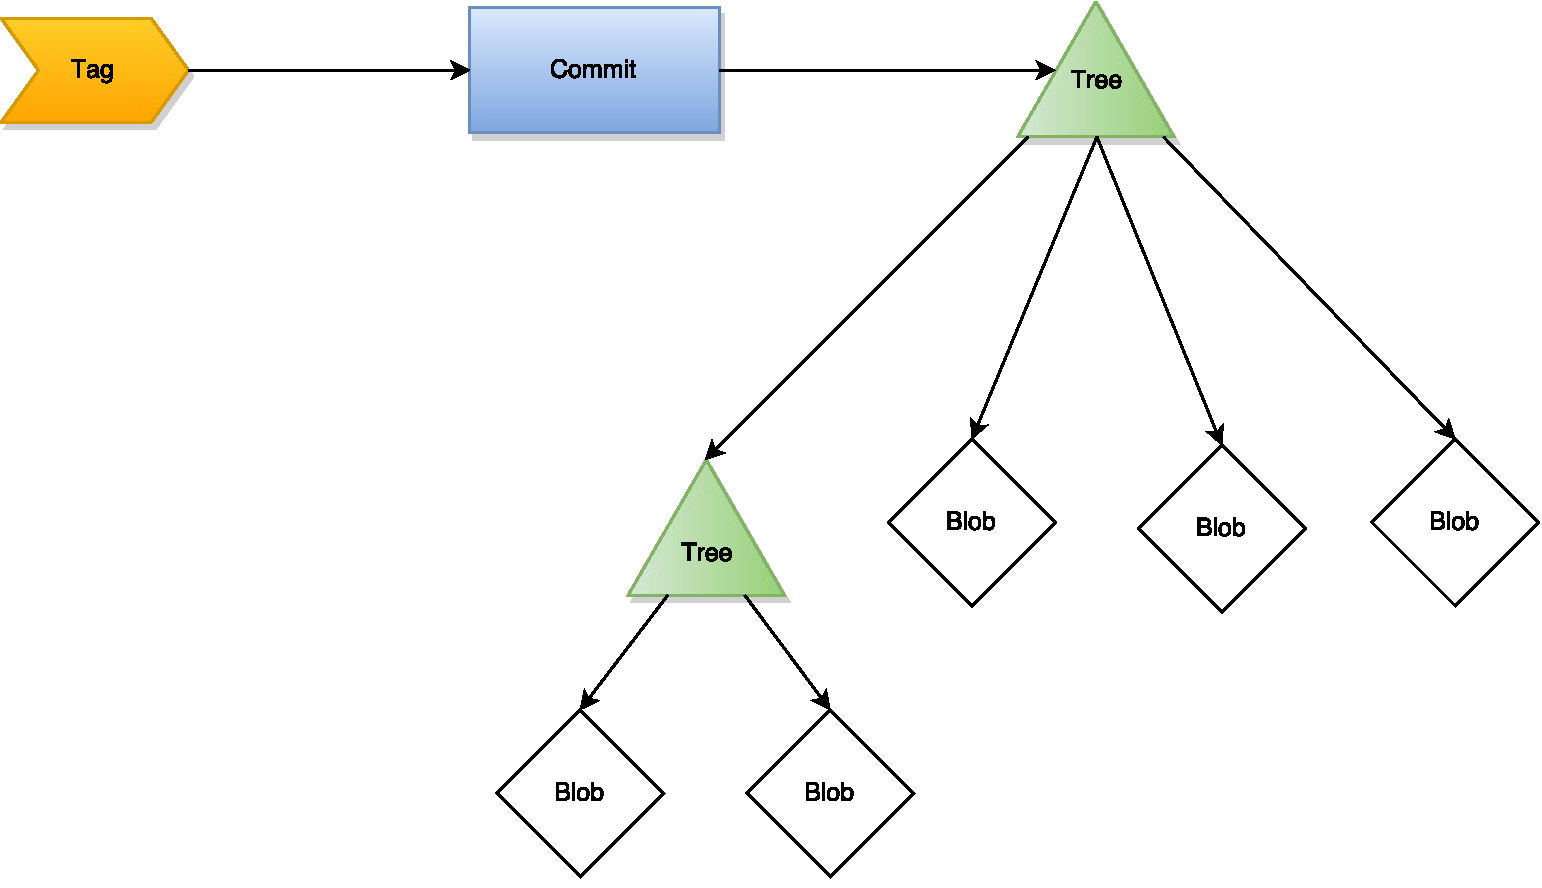
\includegraphics[width=0.7\textwidth]{images/gitobjectmodel}
	\caption{The relationships between Git Objects}
	\label{fig:gitobjectmodeldiagram}
\end{figure} 

Each of these objects will now be discussed in more detail.

\subsection{Blob}
In git a blob is an array of bytes, which can be text or binary data, that is stored in the content-addressable file system. Blobs should not be confused with files as they are just content with no metadata such as filename, in fact if two files are added to git with exactly the same content, and therefore hashcode, they share a blob.

\subsection{Tree}
A tree object in git can be thought of as analogous to a directory in a UNIX file system. For each file in the tree a tuple is stored of the name of file, the hashcode of the blob which contains its content, and a numeric file type code \cite{gitmagic}.

A tree can also contain the names and hashcodes of other trees, allowing for a hierarchical file system, as shown in Figure \ref{fig:gitobjectmodeldiagram}. 

\subsection{Commit}
The commit object type stores information about a snapshot of the blobs and trees in the git repository at a particular time. The information includes the name and email address of the author of changes, the name and email address of the person who made the commit, the UNIX timestamp of the time the commit was made, and a message to explain why changes have been made.

A commit points at one-and-only-one root tree, which contains all the other trees and blobs that form part of that snapshot.

\subsection{Tag}
Tags specify points in history as being important. Typically people use this functionality to mark release points (v1.0, and so on) \cite{gitdocstags}. They contain the hashcode of the 1-and-only-1 commit they point to, a name (such as "v1.0") and a message explaining why the tagged commit is important \cite{gitforcomputerscientists}.

\section{Git Concepts}
Whilst the git object model is reasonably simple it enables some relatively powerful functionality.

\subsection{Branching \& Merging}
All of the git workflows described in section \ref{sec:git} make use of branching. Branches in git allow changes to be made on a separate named track diverged from the main (master) set of changes. This allows for example, in the case of a web browser, a new HTML element to be developed in a branch called 'new-html-element' whilst bug fixes can be made on the main branch. This avoids the complication of multiple different people working on multiple different features on one branch and breaking each others code and focus.

\begin{figure}[h]
	\centering
	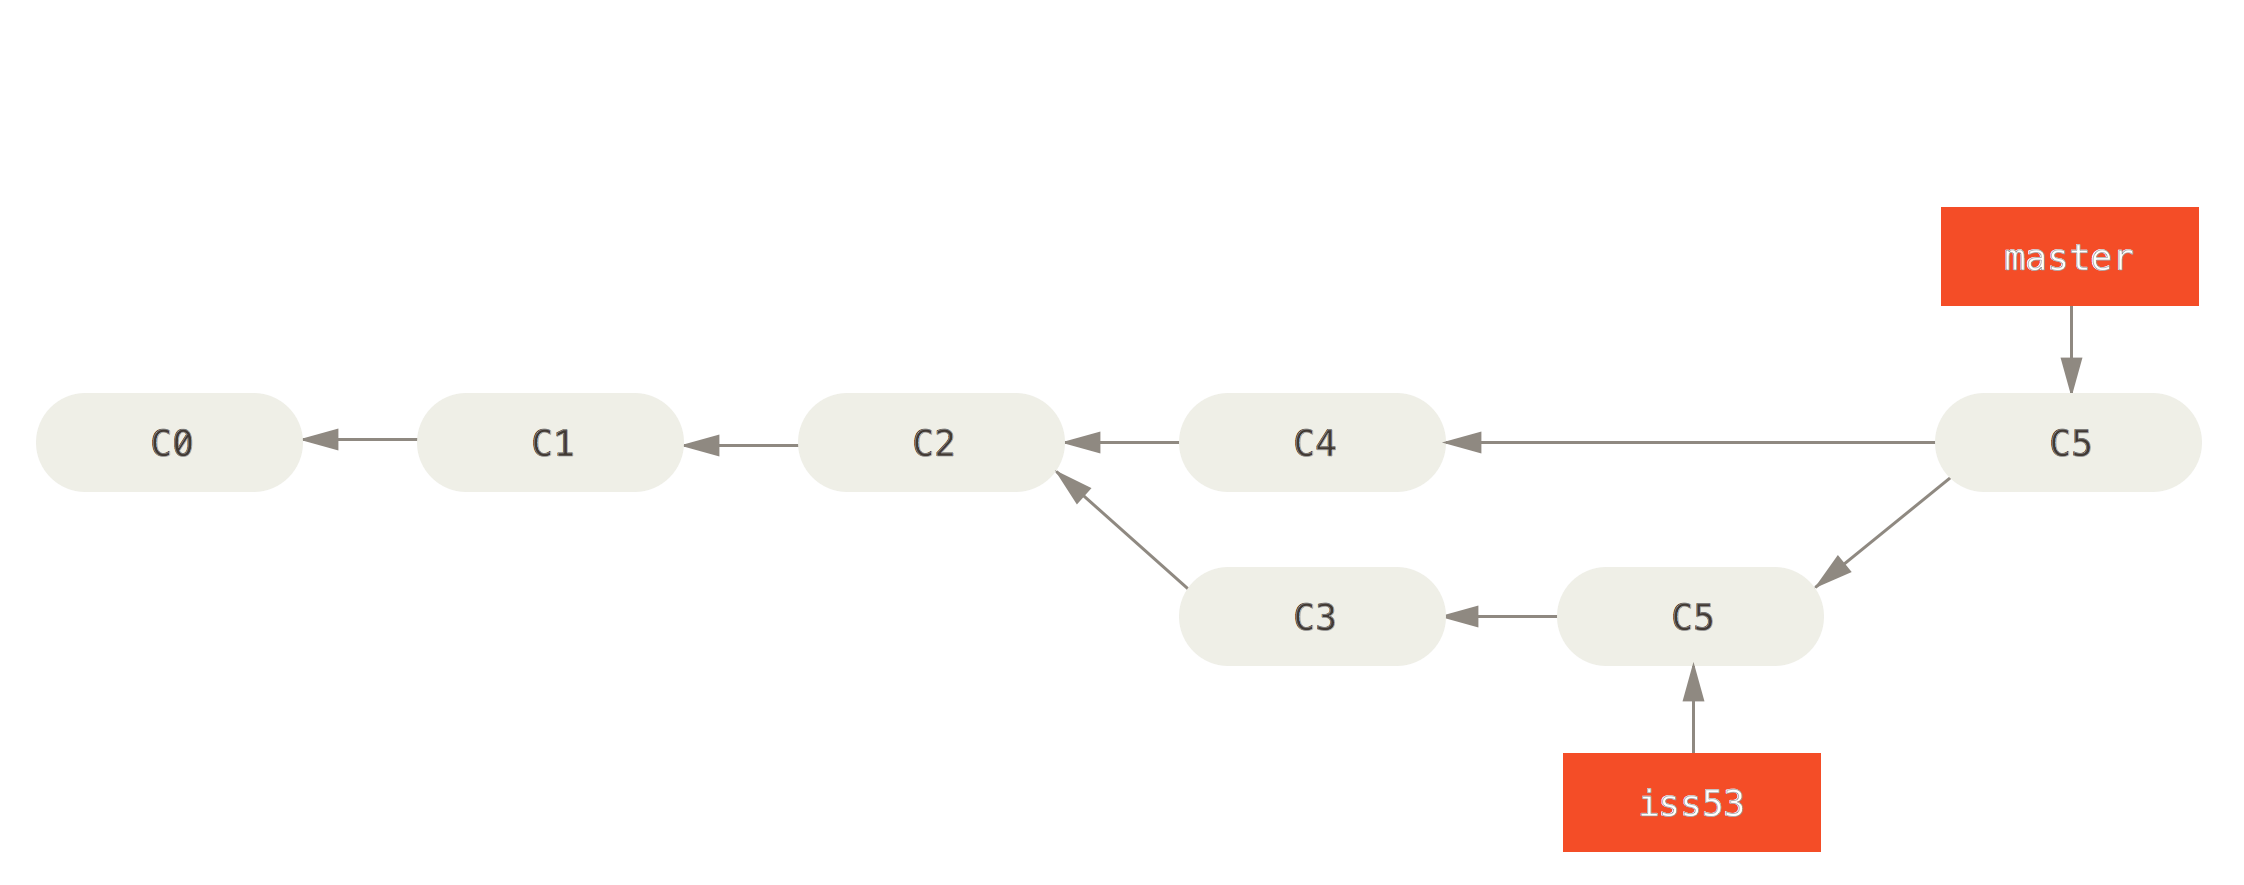
\includegraphics[width=\textwidth]{images/basicbranching}
	\caption{A Simple Branching Scenario \cite{gitbasicbranching}}
	\label{fig:gitbranching}
\end{figure} 

Once work on a branch is complete its changes can be merged into the main branch, or any other branch. When this is done a commit is made, called a 'merge commit' to keep track of the event, in Figure \ref{fig:gitbranching} 'C2' is a merge commit.

\subsection{Forking}
Forking isn't a command in git, or indeed an object type, but rather a concept about how to copy and add to repositories. In the forking workflow \cite{gitcomparingworkflows} a repository is cloned, and committed to as if it was a branch, before pushing changes 'upstream' to the original repository. Often pull requests are required for contributors who do not have direct write access to the original repository.

\section{Existing Git Analysis Tools}
\label{competitors}
% Section on literature pertaining to accessing git information
	% e.g. http://www.researchgate.net/publication/279058070_Gitana_a_SQL-based_Git_Repository_Inspector
	% Some info on gitinspector
	% Conclusions drawn from the literature
		% Primarily, there isnt many projects doing this. The SQL one has some drawbacks, etc.
There hasn't been any previous work on interacting with git through modelling, however there have been several pieces of software developed to allow users to extract information from their git repositories.

\subsection{Git Inspector}
Git Inspector is described as a statistical analysis tool for git repositories. The default analysis shows general statistics per author, which can be complemented with a timeline analysis that shows the workload and activity of each author \cite{gitinspector}.

\begin{figure}[h]
	\centering
	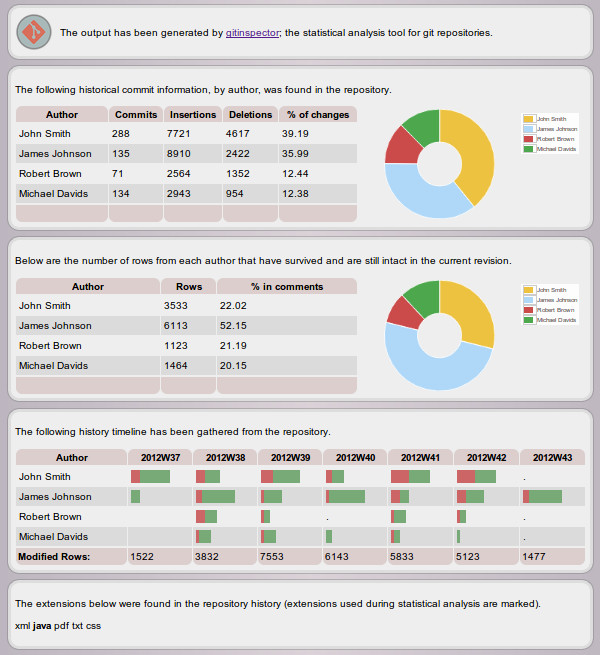
\includegraphics[width=0.4\textwidth]{images/gitinspector}
	\caption{A Sample HTML output from GitInspector \cite{gitinspector}}
	\label{fig:gitinspector}
\end{figure} 

The output from GitInspector is a HTML file with embedded CSS and JavaScript. It is implemented in Python and the queries cannot be edited by a user without editing the program itself.

By reading the code we can see that Git is accessed by GitInpector by issuing commands to the git program installed on the users computer via the system default terminal emulator, the output of git to standard IO is then parsed by Gitinspector. This isn't a particularly efficient way of dealing with the git object model. %Can you reference code?


\subsection{GitStats}
GitStats is a statistics generator for git repositories. It examines the repository and produces statistics from the history of it including most common times of commits, author statistics, total number of files, and total number of tags. Similarly to GitInspector HTML is the only output format \cite{gitstatslinux}. 

\begin{figure}[h]
	\centering
	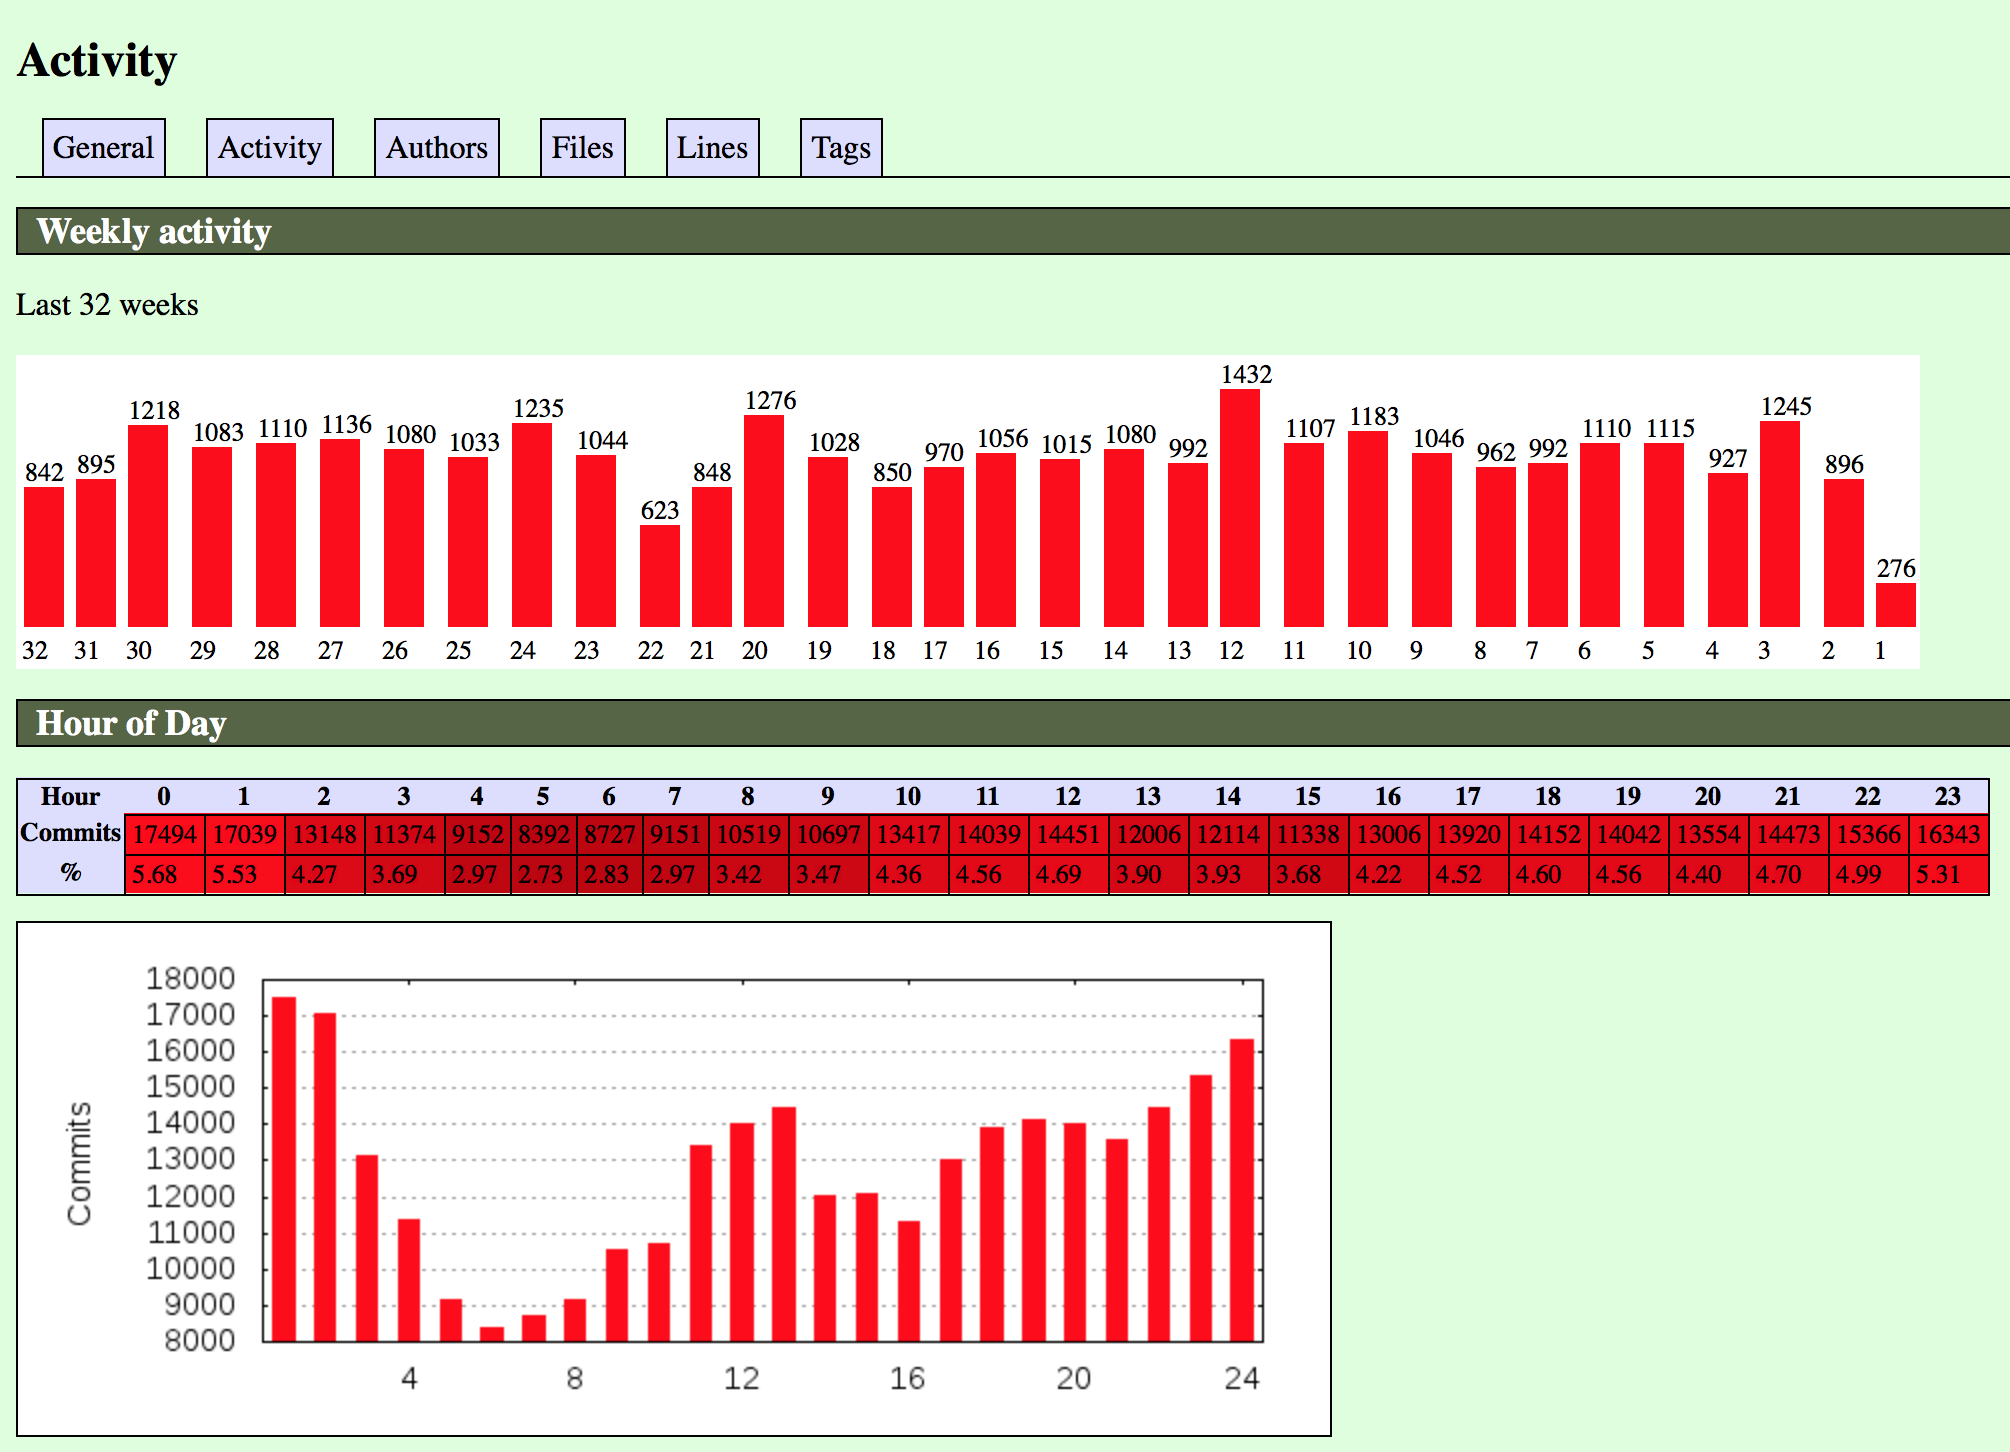
\includegraphics[width=0.8\textwidth]{images/gitstatslinux}
	\caption{A GitStats activity HTML output for the Linux Kernel 2.6 git repository \cite{gitstatslinux}}
	\label{fig:gitstatslinux}
\end{figure} 

Just like GitInspector, GitStats is written in Python and accesses git via a terminal emulator. GitStats provides more statistics than GitInspector however, they too are fixed and cannot be changed by the user without changing the programs code.

\subsection{Github Graphs}
GitHub is a social coding platform built on git \cite{gitpowersgithub}. One of the features of GitHub is Graphs, a set of visualisations of repository statistics \cite{githubgraphs}. Unlike GitStats and GitInspector the statistics are generated on the server-side rather than by a client on their own computer.

\begin{figure}[h]
	\centering
	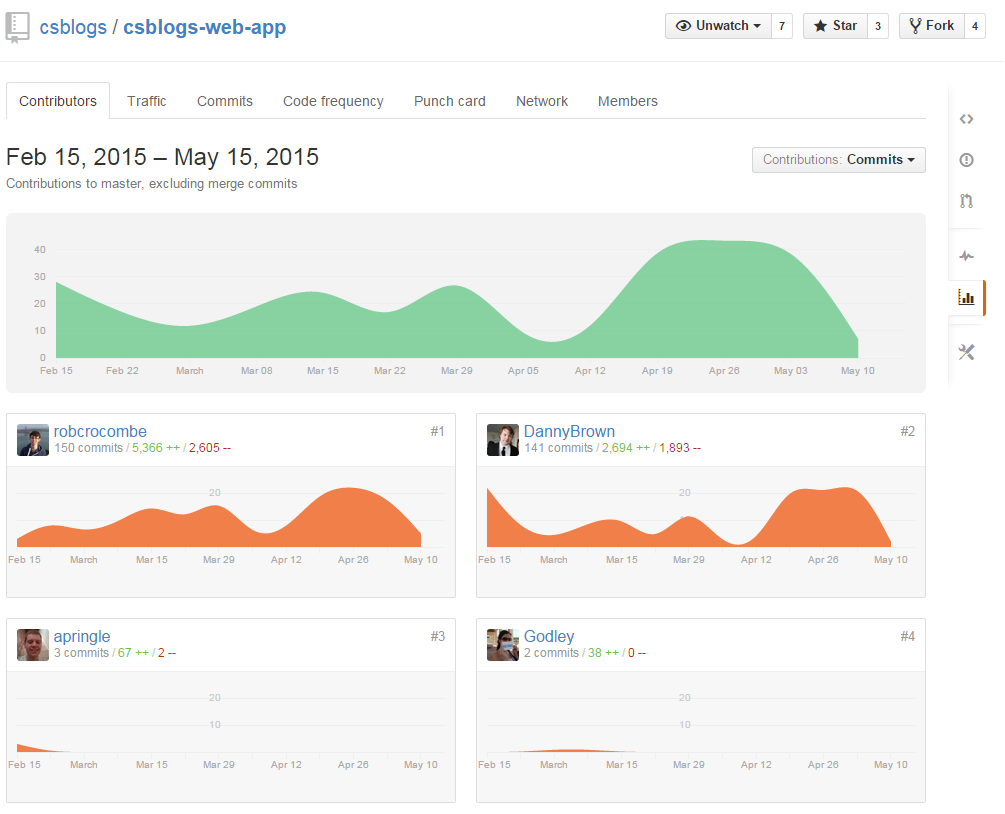
\includegraphics[width=0.8\textwidth]{images/githubgraphs}
	\caption{Some of the graphs which can be generated by Github Graphs \cite{githubgraphs}}
	\label{fig:githubgraphs}
\end{figure} 

Like GitInspector and GitStat the queries ran cannot be altered by the user, but additionally because everything happens on GitHubs servers and the code to generate the reports is closed source users cannot even hack the code to change things.

Unlike the aforementioned packages the results of analysis are displayed in a very modern HTML5 markup, with JavaScript that allows users to select just the information that is relevant to them, e.g. to select information between two dates.

The backend for Github Graphs is developed in Ruby and accesses git via Rugged, a libgit2 wrapper library \cite{rugged}. libgit2 is a portable, pure C implementation of the Git core methods which enables developers to write code which natively interacts with git object databases \cite{libgit2}.

\subsection{Gitana}
Gitana is a system which incrementally exports git information to a relational database which can then be queried via SQL statements \cite{gitana}. One of the things that sets Gitana apart from the other systems is that it allows anyone with knowledge of SQL to write their own queries.

Before any queries can be ran against a repository using Gitana a database has to be built. In order to stop large repositories having to be built into a database often it has support for detecting changes to a git repository and incrementally adding updates. Whist this is good it can still take a reasonable amount of time for a large repository to become query-able the first time an index is built. This can take up to 2 hours per 1000 commits \cite{gitana}.

Thanks to the fact that Gitana uses a Relational Database that can be accessed via SQL it can be integrated with any system that can interact with SQL databases. The developers give examples of integrating with bug tracking software and code reviewing systems.

Gitana itself doesn't have any visual output, it just provides an interface to the data layer, however this allows anyone to build tools on top of it.

\section{Model Driven Engineering}
% More in-depth explanation of modelling
	% What is a model?
	% How do we interact with models?
	% etc?
Model Driven Engineering (MDE) is an approach to tackle the complexity of data, and how it is interacted with, through the use of high level abstractions called models \cite{modeldrivenengineering} and a set of Domain-specific modelling languages and Transformation engines and generators. 

There is some discussion in the literature \cite{basictheorymde} as to the exact definition of a model, it can be thought of as "a simplification of a system built with an intended goal in mind. The model should be able to answer questions in place of the actual system" \cite{precisedefinitionmda} or perhaps more correctly "A model is a description of a (part of) systems written in a well-defined language. A well-defined language is a language with well-defined form (syntax), and meaning (semantics), which is suitable for automated interpretation by a computer" \cite{mdaexplained}.

The author finds that the best way to think of a model is a higher-level abstraction than an object in object-oriented programming language.

A model itself is defined by a metamodel, and a metamodel can be defined by itself \cite{metamodelling}. 

Domain Specific Modelling Languages are specialised languages that enable a user to interact with models in a specific and often highly abstract way, developers use DSMLs to build applications using elements of the type system captured by metamodels and express design intent declaratively rather than imperatively \cite{modeldrivenengineering}.

Transformation engines and generators let the user generate artefacts, such as HTML documentation or source code form their models. As an example a source code generator could be used on a model of a school to create Java class files for every type of person at the school and initialisation code for object instances for each of the students.

MDE platforms, such as Epsilon, often consist of many DSMLs and Generators.

\section{Epsilon}
% About the platform
% EOL, EGX, Etc.
Epsilon, standing for Extensible Platform of Integrated Languages for mOdel maNagement, is a platform for building consistent and interoperable task-specific languages for model management tasks such as model transformation, code generation, model comparison, merging, refactoring and validation \cite{theepsilonbook}. 

The Epsilon Platform can be run as an Eclipse Application or imported into another application as a .jar library file.

Epsilon has a set of domain specific languages and generators for many different tasks based on a core language called Epsilon Object Language or EOL. 

\begin{lstlisting}[caption=An example of EOL code, label=lst:exampleEolCode]
People.all.select(p | p.age > 20 and 
  (p.career = "Computer Scientist" or p.career = "Lecturer"))
\end{lstlisting}

Out-of-the-box Epsilon supports models described in Eclipse Modelling Framework (EMF), XML and CSV formats, but additional model types can be added to Epsilon by use of the Epsilon Model Connectivity Layer.

\subsection{Epsilon Model Connectivity}
The Epsilon Model Connectivity layer enables developers to build plug-ins for Epsilon in order to allow it to access a new type of model through all of its inbuilt domain specific languages and generators \cite{theepsilonbook}.

\begin{figure}[h]
	\centering
	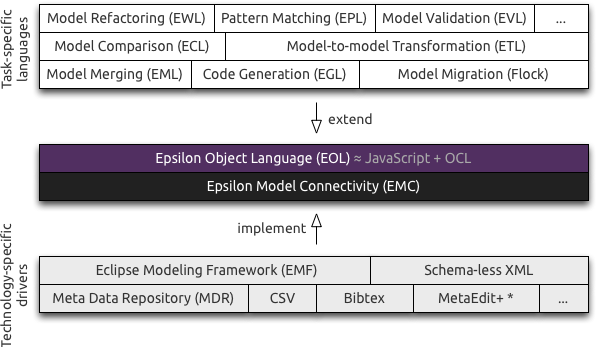
\includegraphics[width=0.8\textwidth]{images/epsilon-architecture}
	\caption{Epsilon Architecture \cite{emcdocs}}
	\label{fig:emc}
\end{figure}

In Figure \ref{fig:emc} it can be seen that implementing the Epsilon Model Connectivity layer allows all the 'task specific languages' to access the models information via EOL. It can also be seen that Epsilons 'built-in' model types are built using the same technology.

The functionality required of an EMC layer is described through the abstract classes which must be implemented in Java, a graphical overview of which can be seen in Figure \ref{fig:imodelinterface}. The \code{IModel} interface describes the formal parameters for functions to control basics such as storing and loading the model, accessing model elements and optionally writing changes to model elements.

\begin{figure}[H]
	\centering
	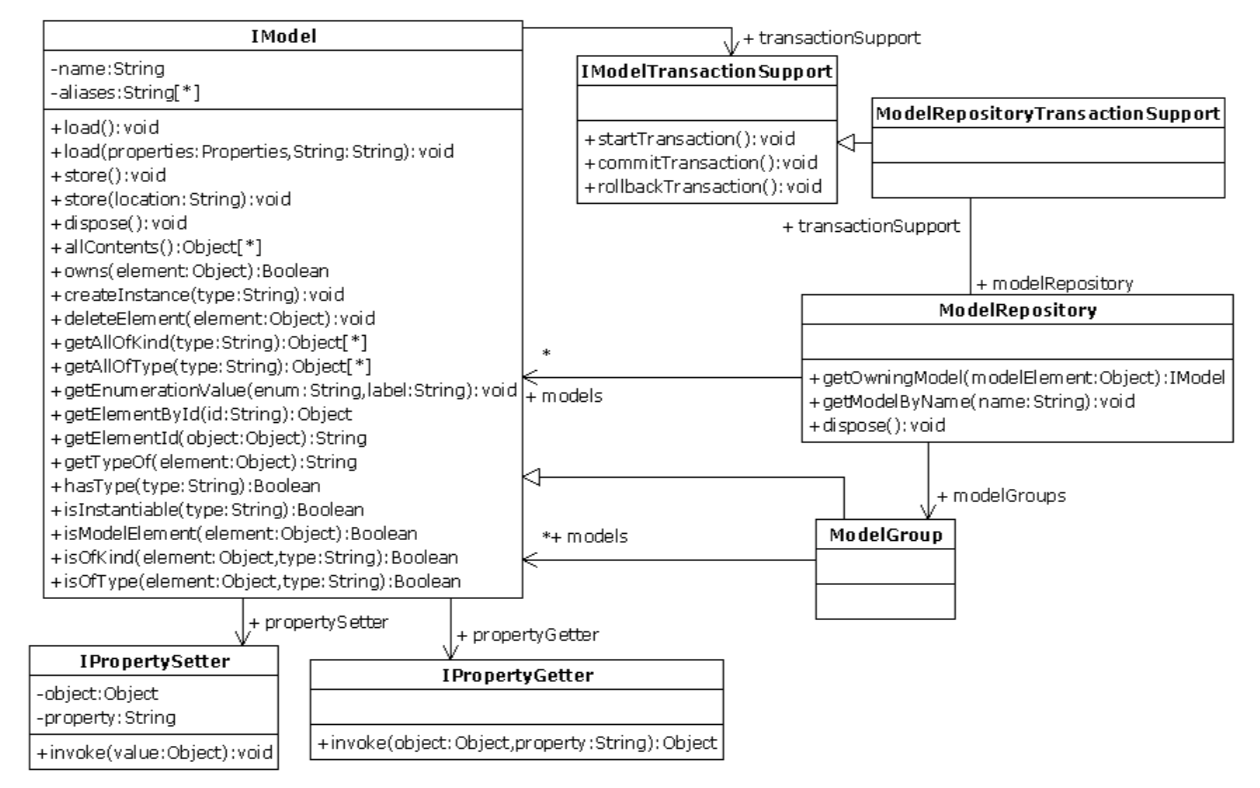
\includegraphics[width=\textwidth]{images/imodel-interface}
	\caption{The IModel Interface \cite{theepsilonbook}}
	\label{fig:imodelinterface}
\end{figure}

\chapter{Requirements}
\label{requirements}

\section{Problem Statement}
\label{problemstatement}
% Statement of Needs
% Stakeholder Identification (whos interested in project and their roles)
	% requirements of these stakeholders
% Breakdown of functional (features) and non-functional (speed, UX) requirements
% Use case diagram
A problem statement outlines the basic issue which the project is trying to solve. An abstract outline of the requirements of the product which could solve this problem will be discussed. This information can then be used to determine stakeholders of the process and guide the requirement solicitation process \cite{problemstatement}.

The problem statement is heavily influenced by the initial project proposal written by the project supervisor \cite{initialproposal}.

\textit{
Git is a popular distributed version control system 	that is widely used both in academia and in industry. Git provides a command-line API through which basic queries can be evaluated against local repositories (e.g. git log) but lacks facilities for expressing complex queries in a concise manner.}

\textit{
The aim of this project is to support such complex high-level queries on Git repositories.}

\textit{
Such an advanced query facility would enable the development of advanced Git repository analytics and visualisation services (e.g. using Epsilon's EGL as a server-side scripting language).}

\section{Stakeholder Identification}
\label{stakeholders}
A stakeholder is a person or organisation who influences a system’s requirements or who is impacted by that system \cite{stakeholders}, because the stakeholders influence the requirements they must be identified before requirements are written in order for the requirements to take them into account and be correct.

Direct stakeholders are people whom interact with the computer system directly as a user, whilst indirect stakeholders are those who are otherwise affected \cite{directvsindirectstakeholders}, both will be discussed in detail.

\subsection{Direct Stakeholders}
\label{directstakeholders}
\subsubsection{Git Analysts}
Project managers, team leads or individuals who want to use the software solution to analyse their git repositories using built-in queries or those developed by other people. The main "users" of the system.

\subsubsection{Query Developers}
The developers writing custom queries either for Git Analysts. An individual could be both a query developer and a git analyst, and this is the expected use case. 

\subsection{Indirect Stakeholders}
\subsubsection{Project Managers}
The people in charge of the project for which analysis is taking place. They may want to use the analysis to help them make strategic decisions about the future of the project or determine why things happened the way they did in the past.

\subsubsection{Users of Git Repositories}
Developers and other people who have contributed code or other artefacts to a git repository are stakeholders because it will be their information and work which is being analysed.

\subsubsection{End users of Code Repositories Analysed}
If the git repository for 'My Word Processor' is analysed and this results in an improvement or deterioration to the workflow for that team it could potentially have an effect on the final product and therefore the end users of 'My Word Processor'. 

\subsubsection{Epsilon Users and Developers}
One of the secondary aims of the project, as outlined in section \ref{aimsandobjectives}, is to get more people interested in Epsilon and Model Driven Engineering -- Therefore the Epsilon Developers are key stakeholders. Users of Epsilon could benefit from increased exposure of epsilon to the developer community.

\subsubsection{Project Supervisor and Author}
Both the Project Supervisor and the author of this project are invested in as good an outcome as possible within the limits in terms of time and resources available to the project. 

\section{Roles of Contributors}
The Project Supervisor, Dr. Kolovos, is the lead developer and project maintainer of Epsilon. This position means that he is well suited to representing the interests of Epsilon users and developers. As outlined in the problem statement in section \ref{problemstatement} Dr. Kolovos initially proposed this project, with the intention of being a user himself, and is therefore also a good spokesperson for project managers, users of git repositories and end users of code repositories analysed.

\section{Use cases}
Uses cases are descriptions of interaction scenarios between a system to be designed and users of the system \cite{usecase}. Figure \ref{fig:usecasediagram} shows the relationships between the direct stakeholders of the system outlined in section \ref{directstakeholders} and their associated actions.

\begin{figure}[h]
	\centering
	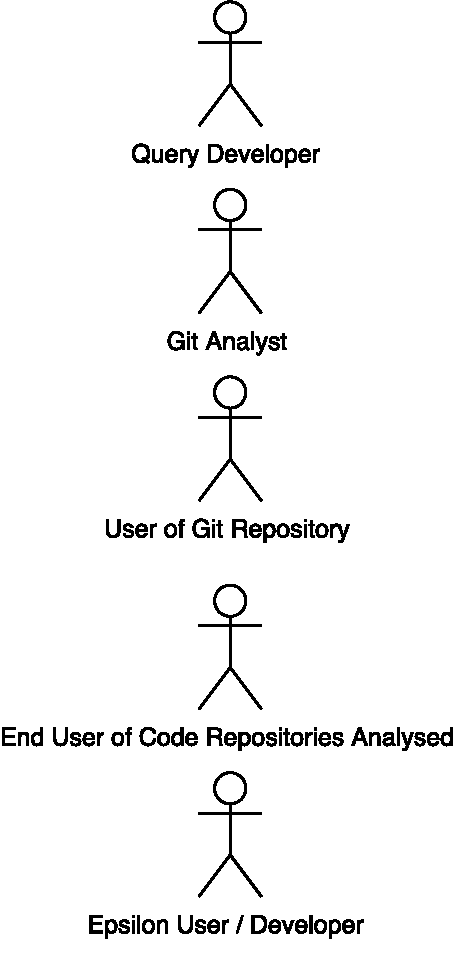
\includegraphics[width=\textwidth]{images/use-case-diagram}
	\caption{EpsilonGit use case diagram}
	\label{fig:usecasediagram}
\end{figure}

\section{Key Capabilities}
\label{keycapabilities}
Through the process of identifying stakeholders in the project, developing a problem statement and having discussions with the project supervisor, who represents the interests of several of the stakeholder groups, a list of key capabilities of the software was written up.

\begin{enumerate}
	\item Ability to query information from the Git Object Model (Commits, Tags, Blobs and Trees) of an arbitrary number of git repositories using the Epsilon Framework and its associated domain-specific modelling languages
	\item Ability to generate HTML and other artefacts from the information in the Git Object Model using The Epsilon Frameworks generators
	\item To have both a high-level API for the commonly used sections of the git system, but access to native code for less commonly used sections that there wasn't time to improve code for
	\item The ability to work on large git repositories in a reasonable time
\end{enumerate} 

These key capabilities are the ones that will be focused on the most during the development stage of the project and will be most important in achieving the aims and objectives of the project outlined in section \ref{aimsandobjectives}.

\section{Stakeholder Requirements}
Stakeholder requirements refer to the requirements of the people identified in section \ref{stakeholders}. They have been decided upon in the same way as the key capabilities of the system. 

Stakeholders have an interest in both the functional and the non-functional requirements of the system. A functional requirement is the requirement of the function of a piece of software \cite{functionalrequirements}, for example "it must be able to add two numbers together", a non-functional requirement is one pertaining to operating cost, performance, reliability, maintainability portability and anything else which doesn't relate directly to the functionality of the program \cite{nonfunctionalrequirements}.

Requirements are laid out in the following style:

\begin{table}[h]
\centering
\begin{tabular}{|p{5cm}|p{5cm}|p{5cm}|}
\hline
\textbf{Identifier} & \textbf{Description} & \textbf{Success Criteria} \\ \hline
A short code to identify the requirement. Type-Function-Number format. E.g. ST-NF-1 would be the first non functional requirement for stakeholders. & A description of what the requirement entails  & What will have to be true for a requirement to have been successfully met. Should be S.M.A.R.T \cite{SMART} \\ \hline
\end{tabular}
\caption{Requirements Style}
\label{tab:requirementsstyle}
\end{table}

\clearpage
\subsection{Functional Requirements}
\begin{table}[H]
\centering
\begin{longtable}{|p{2cm}|p{7cm}|p{6cm}|}
\hline
\textbf{Identifier} & \textbf{Description} & \textbf{Success Criteria} \\ \hline
SH-F-1 & Git Analysts should be able to access all commonly used parts of the git API via a model driven interface &  Git Object Model (Tag, Commit, Tree, Blob) accessible via EOL \\ \hline
SH-F-2 & Git Analysts should be able to access multiple git repositories at once for comparison & Multiple repositories query-able via EOL.  \\ \hline
SH-F-3 & Git Analysts should be able to use generators to develop artefacts from their git repositories & HTML should be able to be produced via EGX files \\ \hline
SH-F-4 & Query Developers should be able to develop epsilon object language code which requires no knowledge of the underlying git repository and can therefore be distributed for others to know about & The model interface should not itself require knowledge of git repository locations \\ \hline
SH-F-5 & Git Analysts should be able to add git repositories to Epsilon Programs and Generators using the Epsilon GUI & An option should be shown to add a git repository as a model in the epsilon GUI. When clicked this should allow the user to name it and select its location \\ \hline
\end{longtable}
\caption{Functional Stakeholder Requirements}
\label{tab:functionalstakeholderrequirements}
\end{table}

\subsection{Non-Functional Requirements}
\begin{table}[H]
\centering
\begin{longtable}{|p{2cm}|p{7cm}|p{6cm}|}
\hline
\textbf{Identifier} & \textbf{Description} & \textbf{Success Criteria} \\ \hline
SH-NF-1 & The code required to develop a query or generate an artefact should be quicker to write than alternative methods & An EpsilonGit program producing identical output as a competitor should require less lines of code \\ \hline
SH-NF-2 & The code required to develop a query or generate an artefact should be easier to learn and remember than alternative methods & An EpsilonGit program producing identical output as a competitor should have a lower cyclomatic complexity \\ \hline
SH-NF-3 & The solution should be able to be run as an Eclipse plug-in for ease of use & The solution should integrate with Epsilon Eclipse to the same level as the built-in EMF model type \\ \hline
SH-NF-4 & Queries developed using EpsilonGit should be equally as performant, or better, than competitors & The average time required to run a query which produces the same output on the same machine should be less for EpsilonGit than for GitInspector \\ \hline
SH-NF-5 & Documentation for the EMC layer of Epsilon should be improved & A document which better explains the steps required to develop an EMC driver should be written and made available to other developers as part of this process \\ \hline
SH-NF-6 & Novel research into the effectiveness of Model Driven Engineering to solve problems in the field of Mining Software Repositories should be produced & The impact of this report should be assessed \\ \hline
SH-NF-7 & The code produced for the solution should be easily maintainable and extendable in the future & There should be low cyclomatic complexity and high class decoupling \\ \hline
\end{longtable}
\caption{Non-Functional Stakeholder Requirements}
\label{tab:nonfunctionalstakeholderrequirements}
\end{table}


\section{System \& Software Requirements}
System and Software requirements are the requirements that don't directly interfere with the user but are required to allow the software to work as intended.
\subsection{Functional Requirements}
\begin{table}[H]
\centering
\begin{longtable}{|p{2cm}|p{7cm}|p{6cm}|}
\hline
\textbf{Identifier} & \textbf{Description} & \textbf{Success Criteria} \\ \hline
SY-F-1 & The software solution must be able to interact with the Epsilon Platform and its set of Domain Specific Languages and Generators & The Software must implement the model reading functions of the \code{IModel} interface provided by Epsilon \\ \hline
SY-F-2 & The software must be able to read information from git & The Software must be able to read all information from the Git Object Model \\ \hline
SY-F-3 & The software must provide information to the Epsilon GUI framework to allow users to select repositories etc & Epsilon GUIs should work in the same way for Git repositories as they do for EMF files \\ \hline
\end{longtable}
\caption{Functional System Requirements}
\label{tab:functionalsystemrequirements}
\end{table}


%Things that need to be done in software to enable what users need
\subsection{Non-Functional Requirements}
\begin{table}[H]
\centering
\begin{longtable}{|p{2cm}|p{7cm}|p{6cm}|}
\hline
\textbf{Identifier} & \textbf{Description} & \textbf{Success Criteria} \\ \hline
SY-NF-1 & The system should allow fast access to git from epsilon & The Software should be as fast as competitors at accessing git \\ \hline
SY-NF-2 & The system should be extensable & The system should provide hooks to easily add new features, particular in an open source fashion \\ \hline
SY-NF-3 & The system should be easy to distribute and install & The system should use an Eclipse Plug-in project to make it a one-click install \\ \hline
\end{longtable}
\caption{Non-Functional System Requirements}
\label{tab:nonfunctionalsystemrequirements}
\end{table}

\chapter{Methodology}
% Used agile TDD based approach, discuss why this was chosen and
Software Development Methodologies are workflow structures for use whilst working on software development projects that aim to structure and simplify the processes involved, with the assumption that this will lead to improved productivity and quality of the final product \cite{useofsystemdevelopmentmethodologies}.

\section{Project Attributes Related to Methodology Selection}
\vspace{-0.2cm}
In this section the project factors affecting the choice of methodology will be outlined.

\begin{table}[H]
\centering
\begin{longtable}{|p{5cm}|p{10cm}|}
\hline
\textbf{Factor} & \textbf{This project} \\ \hline
Number of Developers & 1 \\ \hline
Roles of Developers & Due to the fact there is only one developer they will have to take on all roles; including development, testing, writing documentation and maintenance \\ \hline
Rate of Requirement Change & Whilst the overall aim of the project is unlikely to change, the methods used and therefore the exact requirements are likely to change due to experimentation \\ \hline
Interaction with Stakeholders & One meeting per week takes place between the author and the project supervisor who, as discussed in section \ref{stakeholders}, speaks on behalf of several stakeholders. This could change the requirements of the project or provide valuable assistance in the development process \\ \hline
Time Management & EpsilonGit has to be delivered to a hard, non-negotiable, and reasonably short deadline in which other activities are taking place, as discussed in section \ref{constaints}  \\ \hline
Technical Competency & The developer has had some experience with MDE and Epsilon through a MSc level taught course. He has also developed an IDE with git support previously. Integration with Eclipse, and the more in-depth git concepts are new to him however, which may affect how long it takes to develop solutions \\ \hline
\end{longtable}
\caption{Factors affecting choice of Software Development Methodology}
\label{tab:methodologyfactors}
\end{table}

\section{Agile vs. Process Oriented Methodologies}
Software Development Methodologies can be categorised into two main groups, Process Oriented and Agile \cite{agilesoftwaredevelopementreview}. The Waterfall Methodology, shown in Figure \ref{fig:waterfall}, was one of the first formal Software Development Methodologies and is process oriented. A software engineer has to complete each stage, for the entire product, before moving on to the next one. If any mistakes occur, or requirements change, then all work after that point has to stop and the requirements and any succeeding stages have to be reworked.

Process Oriented methodologies are good because they are easy to understand and follow, even for people outside of the technical process, and provide a paper-trail for managers at each stage. However, their rigid structure can slow the overall process of software development down.

\begin{figure}[H]
	\centering
	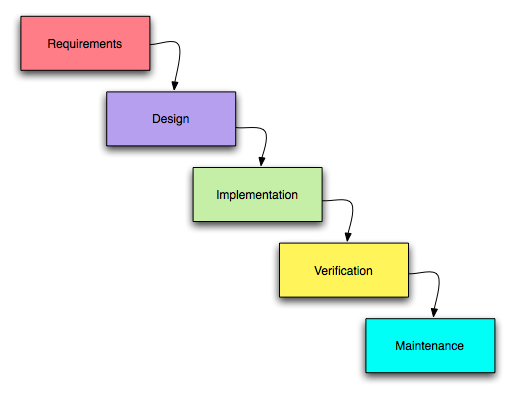
\includegraphics[width=0.6\textwidth]{images/waterfall}
	\caption{The Waterfall Methodology \cite{traditionalwaterfall}}
	\label{fig:waterfall}
\end{figure}

Agile Methodologies are popular both in academia and industry as a lightweight, nimble alternative to process-oriented methods \cite{explainingagile}\cite{agilesoftwaredevelopementreview}. Process based methodologies, such as Waterfall, require that requirements are solicited at the beginning of the process and do not change. As a research project moving goals and constant experimentation is expected and the attributes of agile methodologies are better suited to this kind of work.

Due to the fact that this project will be conducted by a single person, nullifying the need for a paper-trail and non-technical understanding, and is likely to have changing requirements and a need for experimentation it was decided that choosing an Agile methodology was the best route forward.

\section{Considered Methodologies}
There are many popular methodologies which follow the twelve principles bestowed by the Agile Manifesto \cite{agilemanifesto}. Time being a limited resource required that the author investigate only a subset of these. The subset consisted of methodologies the author had previously used or been exposed to, in a hope this might speed up the overall process.

\subsection{Scrum}
SCRUM isn't a methodology in and of itself, but rather a framework for managing the processes of Software Development. It is a team oriented framework that relies on two main characters, a Scrum Master and a Product Owner. A product owner is simply the person who represents the interests of customers or users of the end product, whilst a scrum master is best thought of as a team leader \cite{thescrumguide}.
 
\begin{figure}[H]
	\centering
	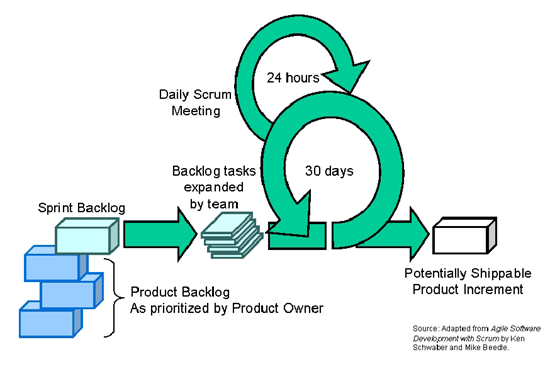
\includegraphics[width=0.6\textwidth]{images/scrum}
	\caption{The Scrum Methodology \cite{scrumdiagram}}
	\label{fig:scrum}
\end{figure}

As seen in figure \ref{fig:scrum} the Product owner develops a list of prioritised changes that are required by the customer, known as a sprint backlog. 

A 'Sprint Plan' takes place in which an amount of these changes are selected by the team to be done in the next sprint -- a 30 day period at which there should be a potentially shippable product with the added changes.

Each working day a 'Scrum Meeting' takes place in which the Scum Master synchronises activities and creates a plan for the days work. Work is given to developers from the backlog of remaining tasks in the current sprint cycle.

At the end of each Sprint a 'Sprint Review' takes place in which the work that took place and the sprint process itself is analysed and discussed by the team members. Items that were decided to be worked on in the Sprint planning stage are categorised as either 'done' or 'not done' by the Scrum Master. Those that are not finished are put back onto the Sprint Backlog to be done in a later sprint.

Scrum is advantageous for a research project such as this one because the product backlog makes it easy to keep track of how the project is progressing and the frequent meetings and discussions aid time-keeping and knowledge sharing between key stakeholders. However, as the project is being tackled by only 1 developer acting as all the characters may be somewhat difficult. 

\subsection{Extreme Programming}
Interaction with the customer and changing requirements at any time, even late in the development cycle, are the key focus points of Extreme Programming (XP) \cite{xpgentalintro}. Changes to the software are made usable and deliverable as soon as possible in order to ascertain early feedback from stakeholders, at a time where changes are the least expensive in terms of time and effort.

\begin{figure}[H]
	\centering
	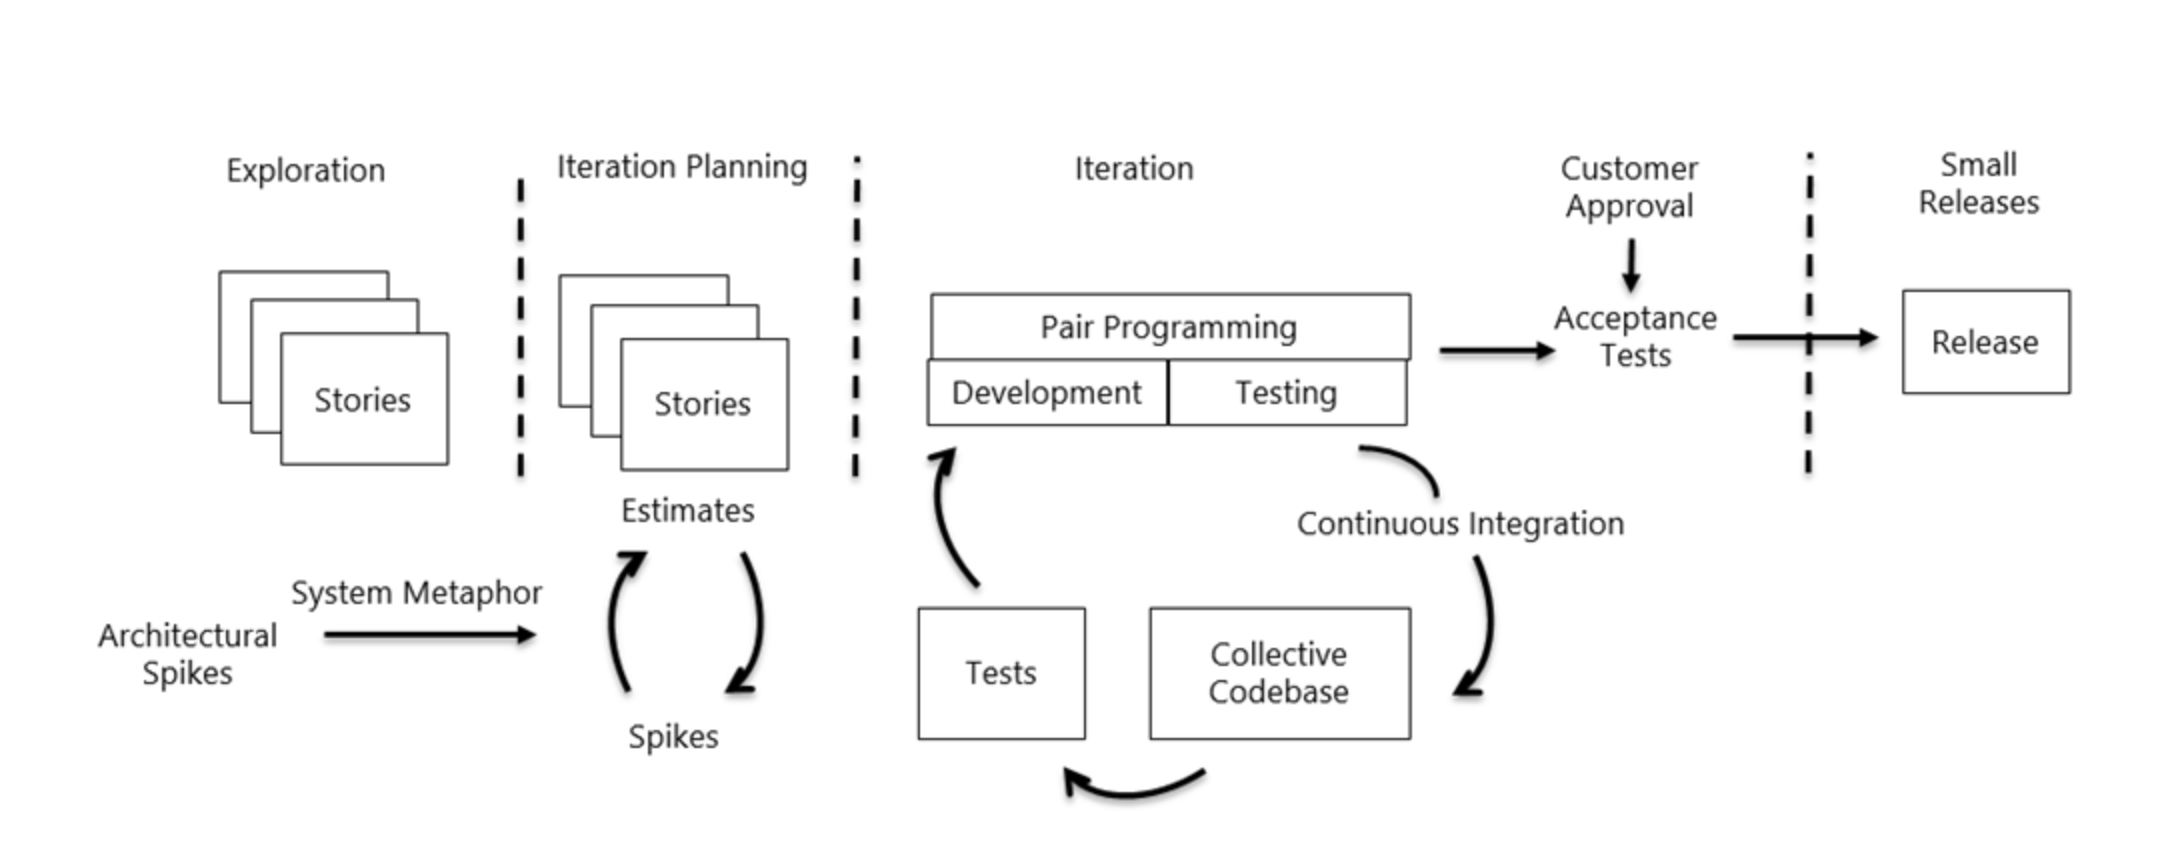
\includegraphics[width=\textwidth]{images/xp}
	\caption{The Extreme Programming Methodology \cite{xpdiagram}}
	\label{fig:xp}
\end{figure}

Figure \ref{fig:xp} shows the four main stages of the XP process. 

In the exploration stage developers work out what is required of the software by soliciting user stories. User stories are simply stories that explain a users need that is to be resolved by the final product, for example "Sally wants to see who committed the most Java code in February". Planning takes place iteratively, in each iteration developers make estimates for how long each story will take to implement and what to focus on next.

The Implementation of the code required for a user story is often written utilising a Test Driven Development methodology in which tests are developed alongside production code \cite{tddxp}. Pair Programming, the process of two developers working side-by-side on the same computer and helping each other solve bugs and develop code, is also often used in order to speed up development and aid learning.

The outcome of the extreme programming model is known as continuous integration (CI). CI is the process of writing and deploying many small changes, along with their required tests, which are often automatically ran to ensure code is ready for a production environment. This continuous integration into a useable product allows for immediate feedback from customers and end-users, which can results in improvements in future releases.

XPs continuous integration, which allows for immediate feedback and rapid changes to requirements suits the needs of this research project well. Additionally the use of Test Driven Development workflows are attractive as they maintain a feedback loop about the quality of the software being written and can alert the developer to any regressions, which are likely given the two complex interfaces being wrangled by the project -- Epsilon and Git.

The downsides to using XP are similar to those of scrum, the methodology is aimed at teams of developers and are therefore not perfectly suited to a one person development team like the one involved in this project.

\subsection{Kanban}
Kanban is a Just In Time (JIT) development process originally developed by Toyota Motors for use in the manufacture of cars that also translates well to Software Development \cite{toyota}.

\begin{figure}[H]
	\centering
	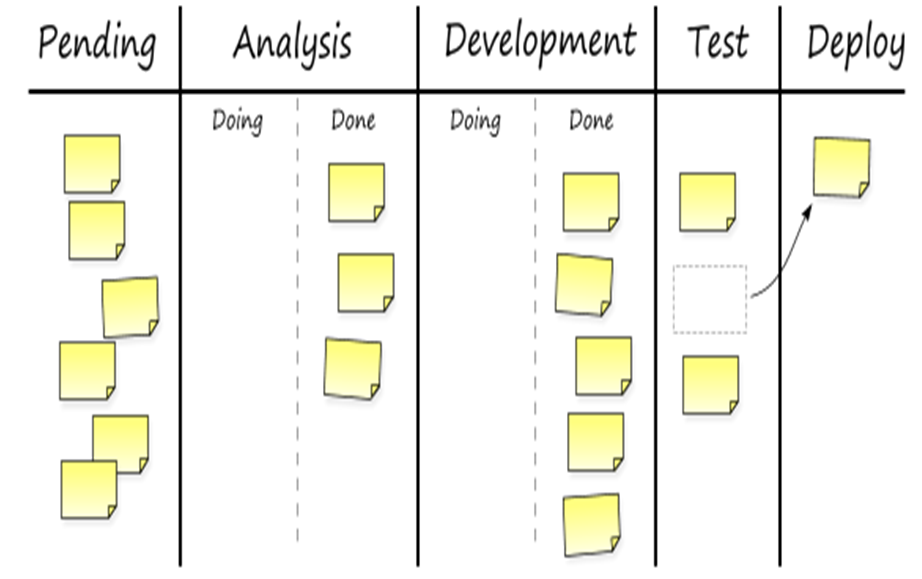
\includegraphics[width=0.6\textwidth]{images/kanban}
	\caption{A Kanban Card \cite{kanbandiagram}}
	\label{fig:kanban}
\end{figure}

Kanban at its most basic is simply a board of tasks, such as the one shown in figure \ref{fig:kanban}, with limits on how many tasks can be in each column at any one time. This stops people and processes from being overworked.

The pending list of features can be ordered by priority by a product owner.

The main advantage of Kanban is its simplicity and ease of use and efficiency through focusing only on what is next to implement rather than having a view over the entire project at any one time. However, the lack of perspective and rigid structure to work could prove to be disadvantageous. 

\section{Selected Methodology} 
\label{selectedmethodology}
None of the methodologies researched matched the requirements of the project perfectly, particularly due to the fact that all of them were built around being used in teams rather than by individuals.

To solve this problem a hybrid agile methodology derived from parts of Scrum, Extreme Programming and Kanban was used. The continuous integration and test driven development ideals from XP were combined with the scrum meetings -- once a week with the project supervisor -- and the focused approach of Kanban.

\chapter{Design}
\label{design}
In this chapter the final design of the EpsilonGit software will be outlined, and the rationale behind many of the design decisions will be discussed. The agile methodology used, as described in section \ref{selectedmethodology}, meant that refactoring of the solution took place often, when deemed necessary to improve the solution -- the rest of this chapter focuses only on the design at the time of writing but includes lessons learnt from the iterative design and implementation process.

\section{System Quality Attributes}
System Quality Attributes (SQAs) are a set of attributes of a proposed system which can be reasoned about in a systematic way in order to aid the design of a systems high-level architecture in an objective way free from bias and hidden assumptions \cite{qualityattributes}.  

To aid the design of the software for this project a subset of the system quality attributes outlined by the Quality Attributes technical report released by Carnegie-Mellon University and a the Microsoft Application Architecture Guide \cite{qualitymicrosoft} were considered based on how relevant they were according to the requirements of the software solution enumerated in chapter \ref{requirements}. They are presented with some methods used to achieve their goals.

In Software Engineering trade-offs occasionally have to be made -- for example making a system more performant may make it harder to maintain in the future or port to new operating systems or platforms -- this reality is reflected in quality attributes. Whilst a single metric cannot accurately describe the effect of trade-offs on a system a simple numeric rank has been assigned to each attribute to signify its relative importance as a time saving device, this is necessary due to the limited time available to the project. The rank of a quality attribute will aid the decision making processes in designing the software if two attributes oppose one another. The numeric ranking ranges from 0, completely unimportant, to 5, critical.

The frequent refactoring and therefore changes to designs of the system based on experimentation made it useful to have a set of Quality Attributes as guiding principles of the development process.

\subsection{Performance}
\textbf{Rating: 4}

Performance refers to system responsiveness: either the time required to respond to specific events, or the number of events processed in a given time interval \cite{performancedefinition}.

Two non-functional requirements of the solution, SH-NF-5 and SY-NF-1, refer to performance as important to the software, in order to compete with competing methods of interacting with git repositories such as GitInspector and Github Graphs. The second objective of this project, outlined in section \ref{aimsandobjectives}, is to develop a solution that is competitive with other solutions in terms of speed therefore this SQA is rated as 4 (important).

In order to develop a performant system lessons learnt from looking at existing git analysis tools in section \ref{competitors}. Gitana took a long time to initially import a git repository to a database, so EpsilonGit will access git data directly as it is needed rather than cache it before use (for example in an EMF model). GitInspector was slow too, but because it read terminal output rather than interfacing with git directly. All of the competing solutions were written in interpreted languages, so using a compiled language may gain some additional speed.

\subsubsection{Methods}
\begin{enumerate}
	\item Interact with Git using a native library rather than by interacting with a git application via Standard IO
	\item Interact with Git directly, rather than by constructing a database or other intermediate representation of data
	\item Develop using a compiled language -- Java
	\item Use the model caching provided by epsilon through the \code{ICachedModel} interface to reduce the amount of disk access and reading of git object data
\end{enumerate}


\subsection{Usability}
\textbf{Rating: 5}

Usability is the ease with which a software system can be used to perform its intended task by its users \cite{usabilitydefinition}. 

Requirements SH-NF-1, SH-NF-2 and SH-NF-3 all relate to making the system easy to use for git analysts and query developers in order to allow more people to use the software and to get more people interested in model-driven engineering in general. The third and fourth objectives of the project, outlined in section \ref{aimsandobjectives}, also highlight the need for reduction of complexity in mining information from Git repositories.

\subsubsection{Methods}
\begin{enumerate}
	\item Integrate with the standard Epsilon user interface system, so that existing epsilon users don't have to learn something new (this is stated in requirement SY-F-3)
	\item Use the Epsilon Object Language and its model specific idioms as an interface to reduce code complexity
	\item Use self documenting method and variable names to aid learning the system
\end{enumerate}

\subsection{Interoperability}
\textbf{Rating: 4}

Interoperability is the level to which a software system integrates with other software systems in its environement; e.g. by using the same data formats, user interface styles or coding conventions \cite{integrationdefinition}.

Interoperability will be particularly important for EpsilonGit as it is effectively a driver between two technologies, Epsilon on one side and git on the other as outlined in requirements SY-F-1 and SY-F-2. However, interoperability with other systems, e.g. an authentication system, is not required so this SQA has been rated as a 4.

\subsubsection{Methods}
\begin{enumerate}
	\item Implement the \code{IModel} interface to integrate with the Model Connectivity Layer of Epsilon (This is a Java interface so Java should be used as the programming language) 
	\item Use the JGit Java Library to integrate with git
	\item Allow access to all features of git through epsilon by subclassing JGit objects to make Model Elements
\end{enumerate}

\subsection{Maintainability}
\textbf{Rating: 3}

The process of changing a software system after initial deployment, or first version, for any reason including the addition of features, bug fixes or optimisation is called maintenance -- the ease and speed at which this can be done is called maintainability \cite{maintainabilitydefinition}. 

This ease with which maintenance can occur is influenced by many factors including use of coding conventions, writing of documentation and use of well-known software patterns, the need for good maintainability for this project is highlighted in requirement SH-NF-7.

\subsubsection{Methods}
\begin{enumerate}
	\item Use third party libraries when appropriate to avoid writing more code then is necessary
	\item Use the Java coding conventions and check them using a Lint program
	\item Use accurate and self documenting variable and method names
	\item Develop documentation
\end{enumerate}

\subsection{Conceptual Integrity}
\textbf{Rating: 3}

Conceptual integrity defines consistency and coherence of the overall design of a system architecture \cite{qualitymicrosoft}. It can be thought of as maintainability but on a design level rather than at the implementation level. 

This would primarily be useful to enable easy extensibility to the software in the future as required by requirement SY-NF-2. 

\subsubsection{Methods}
\begin{enumerate}
	\item Document design decisions
	\item Allow experimentation and extension of code but within the confines of the documented design
	\item Use a similar design to existing Epsilon Model Connectivity packages so as to reduce learning required to contribute to EpsilonGit 
\end{enumerate}

\section{High Level Architecture}
\label{hla}
% Diagram here
\begin{figure}[H]
	\centering
	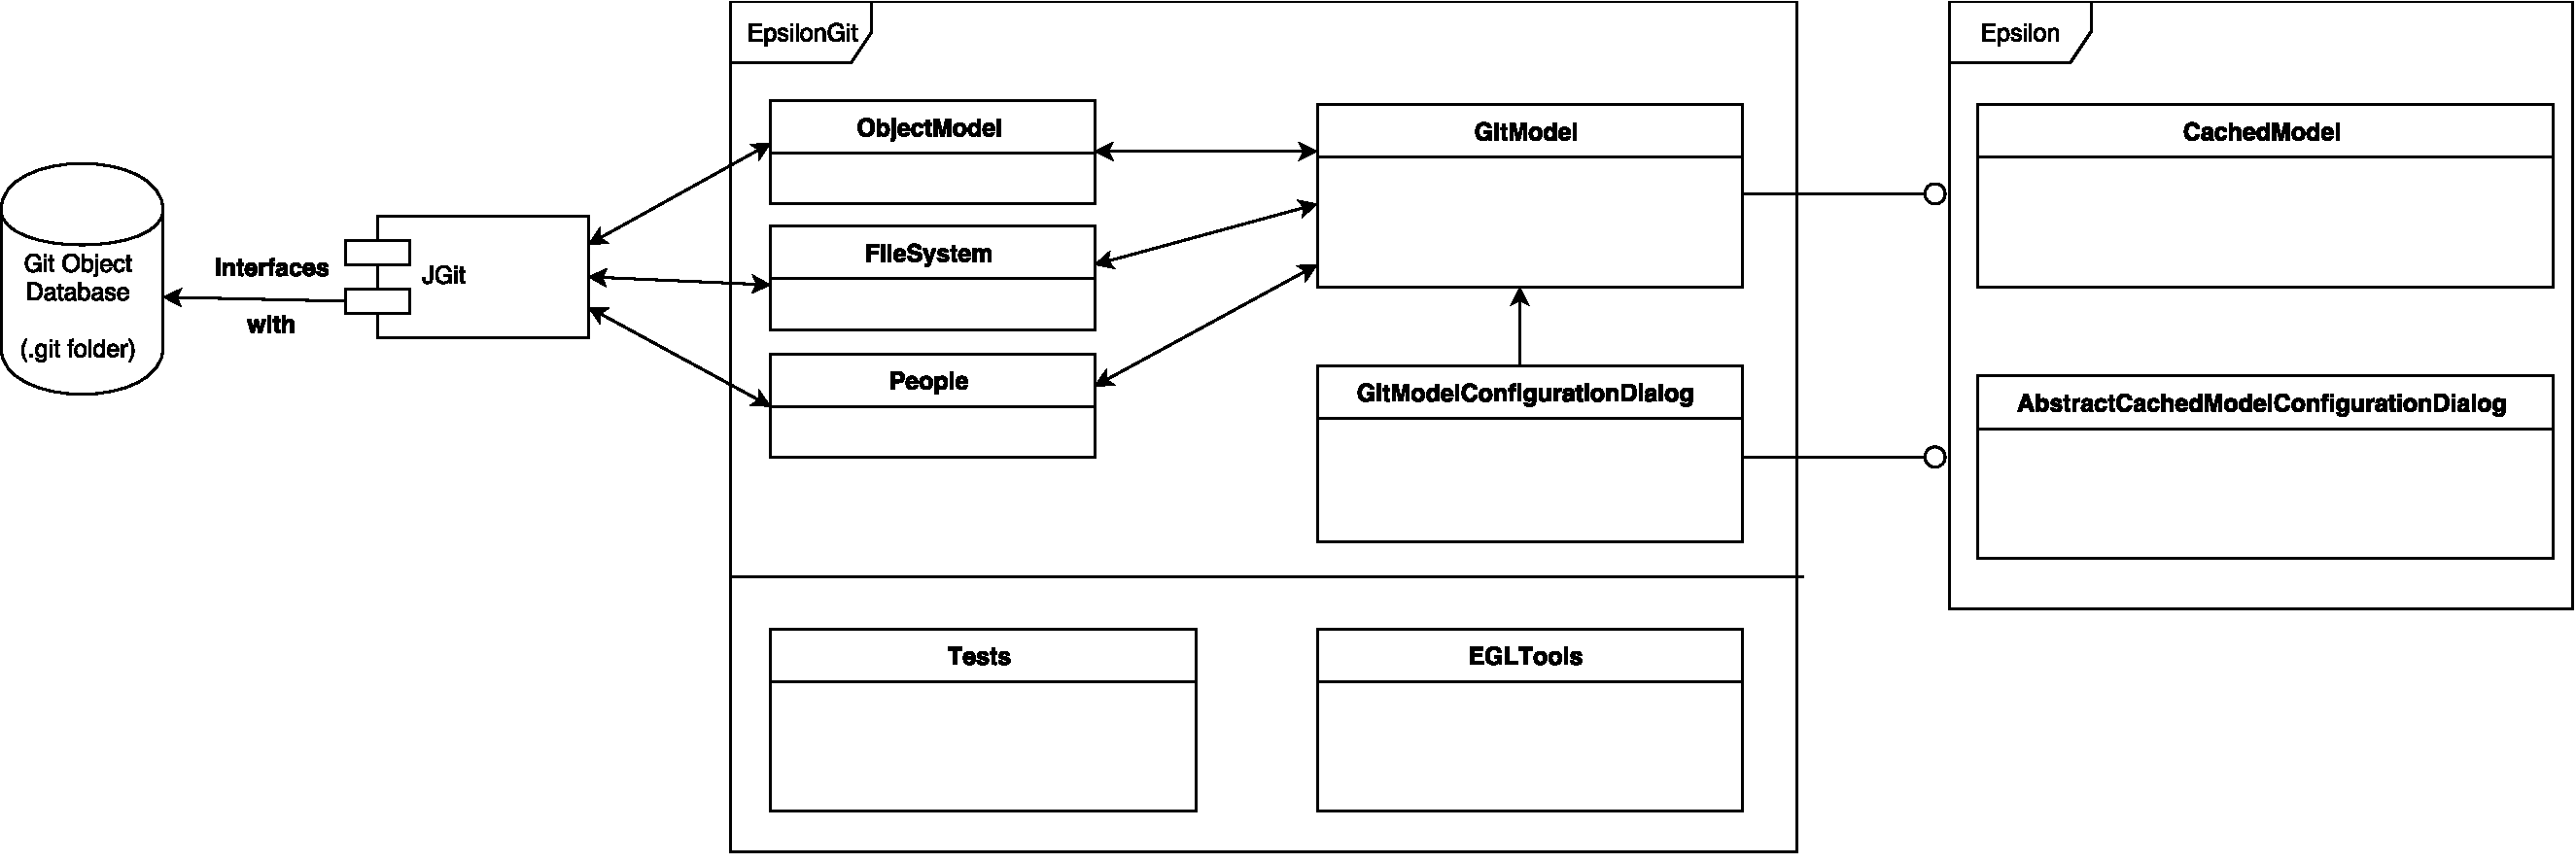
\includegraphics[width=\textwidth]{images/arch}
	\caption{High Level Architecture of EpsilonGit}
	\label{fig:hla}
\end{figure}

Figure \ref{fig:hla} shows the high level architecture design of EpsilonGit and how it interfaces with both Epsilon and Git repositories.

On the left of the diagram a git object database can be seen. A git object database is a directory of files which contains git object model data stored in a binary format. In a standard git setup this directory will be named \code{.git} -- the dot signifying it as a hidden file in UNIX-like systems.

In order to read data from the git object database a Java module called JGit is used \cite{jgit}. Early in the initial design process it was decided that a third-party library should be used to interface with git due to the complexity involved in doing so. 

The main class of EpsilonGit is the \code{GitModel} class which extends the \code{CachedModel} class provided by Epsilon. Extending this class, which implements the \code{IModel} interface allows the program to hook in as a Epsilon Model Connectivity module. Extending the \code{CachedModel} class, rather than \code{IModel} itself, provides caching of objects used by the system after they have been read for the first time, reducing the number of times the Git Object Database has to be read from, therefore improving performance.

The git model provides access to three main types of model elements. Tree, Blob, Commit and Tag git objects are part of the ObjectModel module. The People module provides access to model elements representing Authors and Committers. Finally the FileSystem module allows users to interact with the git object model on a per-file basis -- allowing them to, for example, get all commits associated with a certain file name -- despite git not having knowledge of files, just blobs and trees. The FileSystem module was included to aid to usability of the system for those not familiar with gits internals.

In order to allow a \code{GitModel} object to be created from the user interface provided by Epsilon Eclipse for cached models a class which implemented the abstract base class \\ \code{AbstractCachedModelConfigurationDialog} is included in the design.

Separate from the EpsilonGit system itself, but part of the project, are the two modules at the bottom of figure \ref{fig:hla}. 

Tests consists of a JUnit \cite{junit} unit testing module developed in a test-driven development style alongside EpsilonGit itself. It contains unit tests to test individual methods with different input data and edge cases and integration tests designed to test the aggregation of methods. Validation tests, to ensure the requirements of the software are being met, are also included by way of test EOL files. This is explained in more detail in chapter \ref{testeval}.

EOLTools is a small module designed to make 	developer artefact generators for Git data easier, for example it includes methods which assigns a random colour to each Person, committer and/or author, in a repository for use in graphs or other visual media.

\section{Component Designs}
\subsection{GitModel}
\begin{tcolorbox}
\textbf{Requirements addressed:}  SH-F-1, SH-NF-3, SY-F-1, SY-F-2
\end{tcolorbox}

As described in section \ref{hla}, the \code{GitModel} is the class which implements all of the functionality required by the Epsilon Model Connectivity layer to allow Epsilon to treat a git repository as a model/structured artefact. It does this by implementing the relevant methods provided by the \code{IModel} interface indirectly by extending the \code{CachedModel} class.

\subsubsection{IModel Interface}
The \code{IModel} interface allows Epsilon to hook into the data provided by git, in order to do this it provides the methods outlined and described in Table \ref{tab:imodel}. EpsilonGit doesn't implement all of the methods as, due to the scope of the project, the ability to modify or delete model elements is not required -- the project only requires reading of a git repositories data to provide querying and analysis functionality.

\begin{table}[H]
\centering
\begin{longtable}{|p{3cm}|p{6.5cm}|p{5.5cm}|}
\hline
\textbf{Method Name} & \textbf{Description} & \textbf{Implemented} \\ \hline
allContents() & Returns a collection containing all of the objects contained by the model & Yes \\ \hline
createInstance() & Initialises a new instance of a model & No - New git repositories cannot be made by EpsilonGit. This is outside the scope of the project \\ \hline
deleteElement() & Deletes an element of the model & No - EpsilonGit is read-only \\ \hline
getAllOfKind() & Return a collection of all objects of a specified kind. E.g. All people and any subclasses of people & Yes \\ \hline
getAllOfType() & Return a collection of all object of a specified type. No subclasses &  \\ \hline
getElementById() & Each model object has an ID. This method returns whichever element is associated with the provided ID & Yes \\ \hline
getElementId() & Gets the ID of any given element. For object model types this is their hash code & Yes  \\ \hline
getTypeNameOf() & Returns the name of any owned object's class & Yes \\ \hline
hasType() & Determines if the model supports a given type & Yes \\ \hline
isInstantiable() & Determines if Epsilon can instantiate a new version of that model & No - EpsilonGit is read only \\ \hline
load() & Load the model from storage & Yes \\ \hline
store() & Save the model to storage & No - As no changes can be made in EpsilonGit nothing needs to be saved back to disk \\ \hline
owns() & Determines if a model element is owned by the model & Yes \\ \hline
setElementId() & Sets the ID of an Element & No - IDs like other data are read only \\ \hline
\end{longtable}
\caption{Methods of the \code{IModel} interface \cite{imodeljavadoc}}
\label{tab:imodel}
\end{table}

\subsubsection{Caching}
\label{caching}
The decision was made to extend the \code{CachedModel} class, rather than implement the \code{IModel} interface directly, as it adds caching functionality, meaning that data access times decrease for EOL programs that access model elements more than once. The increased performance this allows helps to address requirements SY-NF-1 and SH-NF-4. \\

\begin{lstlisting}[caption=EOL Code benefiting from caching, label=lst:caching]
Commit.all.size().println();
for(commit in Commit.all) {
	(commit.getFullMessage()).println();
}
\end{lstlisting}

Listing \ref{lst:caching} shows a simple EOL program which prints out the number of commits in a git repository and then prints out message of each commit. In this example all the commits of the git repository are read into the system on line 1, when they are first required. If the system was not using \code{CachedModel} then the same commits would be read in from scratch on line 2 -- which in the case of some large repositories could mean reading several thousand object database files. Using \code{CachedModel} retains the commits in memory, solving this performance bottleneck. For situations where caching may not be appropriate, for example where there are more commits then may fit in memory, then the user can turn caching off via their model configuration dialog.

\subsection{ObjectModel}
\begin{tcolorbox}
\textbf{Requirements addressed:}  SH-F-1, SH-NF-1, SH-NF-2, SY-F-2
\end{tcolorbox}
The ObjectModel module is a java package which contains representations of the git object model types -- Tree, Blob, Commit and Tag -- that can be used as model elements in Epsilon accessed via the GitModel class. 

\subsubsection{Subclassing JGit Types}
In order to ensure that all of the git system is available to EpsilonGit users it was decided that the Model Elements representing git objects should be subclasses of the associate JGit type. Table \ref{tab:subclassing} shows the parent class of each object model model element.

\begin{table}[H]
\centering
\begin{longtable}{|p{7.5cm}|p{7.5cm}|}
\hline
\textbf{Model Element} & \textbf{Parent Class}  \\ \hline
Commit 	& jgit.revwalk.RevCommit \\ \hline
Tag 	& jgit.revwalk.RevTag \\ \hline
Tree 	& jgit.revwalk.RevTree \\ \hline
Blob 	& jgit.revwalk.RevBlob \\ \hline
\end{longtable}
\caption{Object Model JGit subclassing}
\label{tab:subclassing}
\end{table}

Extending these JGit types means that the author doesn't have to reimplement methods like \code{commit.getFullMessage()} which saves time -- the main constraint on this project. It also means that all functionality provided by JGit is available to users through the model driven interface -- meaning a prospective user doesn't have to decide between all of JGits features and the ease of development provided by the EpsilonGit model driven approach.

The downside of subclassing the JGit classes directly is that they were not developed with the intention of being used in a modelling environment, and therefore some of the methods either don't make sense in this context or cannot be used. An example of this is that some methods require an integer constant as a parameter. These constants are public fields of JGit classes, however Epsilon doesn't allow access to fields directly and requires the use of getter and setter methods. This meant that even though a method could be accessed through Epsilon it was in fact unusable and a replacement or override had to be developed.

\subsubsection{Helper Methods}
The third key capability of EpsilonGit, outlined in section \ref{keycapabilities}, is that it provides a high level API for the most common parts of the git system in order to aid rapid, easy development of query and analysis EOL programs.

To this end each of the object model elements have methods to make development easier. Table \ref{tab:helpermethods} displays a subset of the features added by these helped methods.

\begin{table}[H]
\centering
\begin{longtable}{|p{2cm}|p{4.5cm}|p{8.5cm}|}
\hline
\textbf{Element} & \textbf{Method} & \textbf{Description}  \\ \hline
Commit & isRoof & Determines if a commit is the roof (first) commit in a repository \\
& isHead() & Determines if a commit is the last (most recent) commit in a repository \\
& isMergeCommit() & Determines if a commit is the product of merging two branches \\
& getCommitCalendar() & Returns a Java calendar object representing time rather than a raw UNIX time integer, making it easier to compare dates and times \\
& getDifferenceFromParent() & Returns a collection of differences (modifications, deletions, additions) from the previous commit \\ \hline
\end{longtable}
\caption{Object Model Helper Methods}
\label{tab:helpermethods}
\end{table}

\subsection{FileSystem}
\begin{tcolorbox}
\textbf{Requirements addressed:} SH-NF-1, SH-NF-2, SY-F-2
\end{tcolorbox}
As explained in section \ref{gitobjectmodel}, git has no concept of files -- instead it keep track of blobs of data which can be associated to a name in a tree.

This subtle difference is actually quite important. For example, if a user was to assume a Blob was analogous to a file then they might start to make assumptions about the number of files in a repository by counting the number of blobs, even though one blob can represent many files with the same data but different file names or not be associated to a file at all (blobs can be added to git without a corresponding name in a tree).

In order to make development of query and analysis tools easier for people with little knowledge of the internals of git it was decided that a \code{GitFile} class should be developed that allowed people to think in terms of files rather than blobs and trees. 

The \code{GitFile} class provides the following functionality:

\begin{enumerate}
	\item Allows a user to determine if a file exists in the working directory
	\item Keeps track of commits in which the file was 
	\begin{enumerate}
	\item Added to the repository
	\item Modified
	\item Deleted
	\item Copied
	\item Renamed
	\end{enumerate}
\end{enumerate}

\subsection{People}
\begin{tcolorbox}
\textbf{Requirements addressed:} SH-F-1, SH-NF-1, SH-NF-2, SY-F-2
\end{tcolorbox}
People in git are represented in two forms -- authors and committers -- however, there is no one type of object which contains their information. Rather, their information is spread out in different areas of the git object model. 

The author anticipates that git analysts would be particularly interested in the analysis of individuals within a team, therefore it was important to make accessing information about people as simple as possible. 

In order to do this 3 classes are required:
\begin{enumerate}
	\item \code{Author} which represents someone who has developed code or another artefact which is in the repository
	\item \code{Committer} which represents someone who has committed code to the repository
	\item \code{Person} which is an abstract class which can be used to reason about both committers and authors
\end{enumerate}

In git a person can be an author, a committer or both and these classes allow that flexibility. The \code{Person} class in particular makes it easy to just query all people involved in a project, regardless of their role within it.

Having the people model elements means that query developers don't have to parse out information from every Commit and Tag which contains information about a human, that is all done for them by EpsilonGit.

\clearpage

\subsection{Configuration Dialog}
\begin{tcolorbox}
\textbf{Requirements addressed:} SH-F-5, SH-NF-3, SY-F-3
\end{tcolorbox}

In order to make epsilon git easy to use it integrates with the graphical user interface of Eclipse Epsilon. This allows users to specify the location of their git repositories and whether or not they would like to use the caching mechanism explained in section \ref{caching} without having to write code or use a command-line.

\begin{figure}[h]
	\centering
	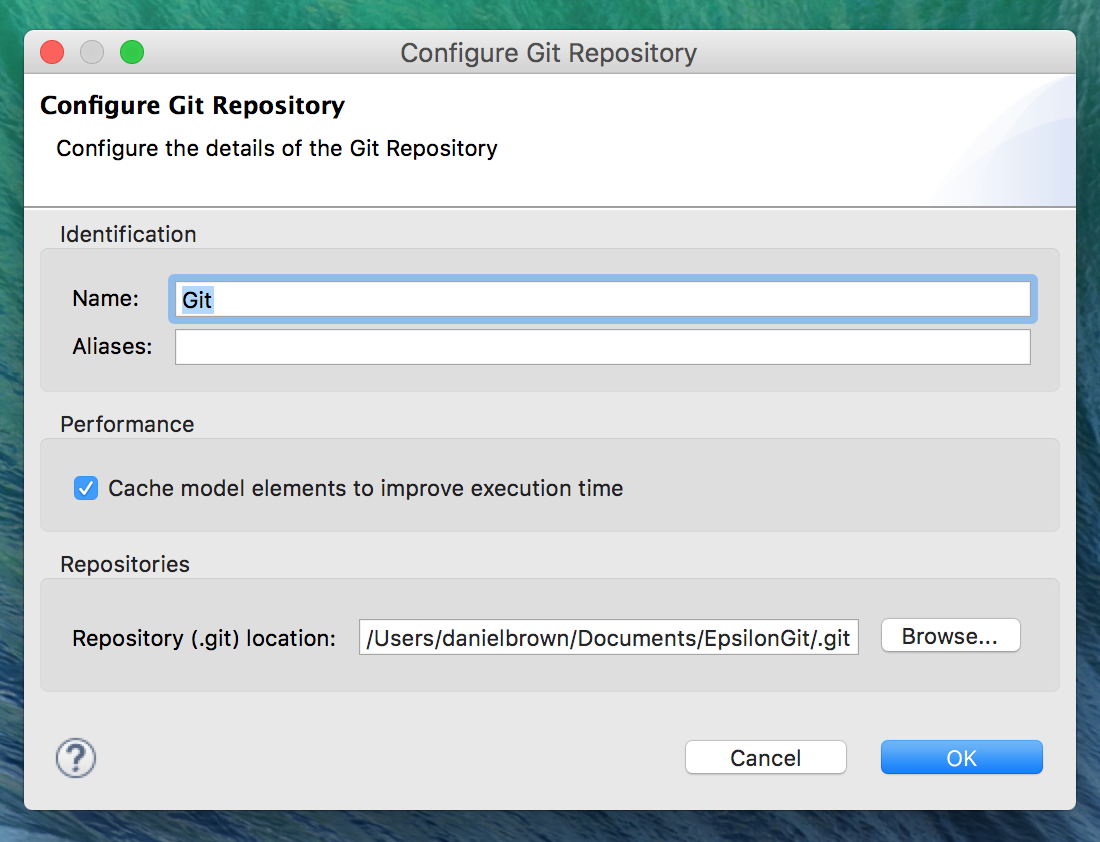
\includegraphics[width=0.6\textwidth]{images/configurationdialog}
	\caption{EpsilonGit configuration dialog}
	\label{fig:configurationdialog}
\end{figure}

In order to be able to provide a Configuration GUI the configuration dialog has to implement the \code{AbstractCachedModelConfigurationDialog} provided by Epsilon.

It was decided that the configuration dialog box would ask the user to provide the location of the object database of their git repository itself, rather than the root working directory of their git repository as it is possible for git repositories to contain other git repositories or have their object database named something other than \code{.git}, so asking for the object database directly avoids some edge cases at a small cost to ease of use as by default these object database directories are hidden.

\chapter{Implementation}
In this chapter the implementation details of EpsilonGit will be explained including information about how to set up EpsilonGit for use on the readers machine, the structure of the projects code and the environment used for development purposes.

\section{Preparing the Development Environment}
The design shown in chapter \ref{design} shows that several different tools and libraries are part of the EpsilonGit system development process. In this section the tools installed in order to complete the project will be discussed.

\subsection{Integrated Development Environment}
There are several commercial and open source IDEs available which allow their user to write, compile and run their Java code, however as the project is being developed to integrate with the Epsilon Modelling Platform which is a Eclipse Foundation product and integrated into the Eclipse IDE itself, thus requiring the EMC layer to be written as an Eclipse Plug-in project, it only makes sense to use Eclipse to write the projects code.

To begin with the publicly available latest release version of the Epsilon Eclipse package was used -- version 1.2 of Epsilon with Eclipse 4.4 Luna. However, mid-way through the project the author hit Epsilon Bug \#341481 \cite{epsilonbug}. At this point the author updated to the latest interim release in which this bug had been fixed -- this required the editing of one line of code. 

\section{Project Structure}
The EpsilonGit project is structured as 4 Eclipse Plug-in projects, one for each of the main modules discussed in the design chapter and displayed in the EpsilonGit frame of figure \ref{fig:hla}. Eclipse Plug-in projects were used in order to maintain compatibility with Epsilon. These projects are:

\begin{enumerate}
	\item \code{org.eclipse.epsilon.emc.git} \\ The main EMC driver project
	\item \code{org.eclipse.epsilon.emc.git.dt} \\ The project for integrating with Epsilons user interface 
	\item \code{org.eclipse.epsilon.emc.git.tests} \\ The project containing JUnit tests for the EMC driver
	\item \code{org.eclipse.epsilon.emc.git.tools} \\ The project containing the EOL tools described in chapter \ref{design}
\end{enumerate}

The tests were originally contained in the main EMC driver project, however it was decided that they should reside in their own project to make a clear line between what was production code and what was auxiliary testing code. Encapsulating the tests in their own project also meant it would be easier to add tests for the tools and user interface projects in future.

The \code{dt}, \code{tests} and \code{tools} projects each contain only one Java package, of the same name, however the main EMC driver project contains several Java packages which encapsulate different functionality in order to aid the organisation and therefore maintainability of the code.

\clearpage

The packages that make up the main EMC driver are:

\begin{enumerate}
	\item \code{org.eclipse.epsilon.git} \\ Contains the main class, \code{GitModel.java} , which implements the \code{IModel} interface and \code{GitCalendar.java}, a class which provides the helper methods for working with commit times
	\item \code{org.eclipse.epsilon.git.objectmodel} \\ Contains the classes which provide access and helper methods for the git object model
	\item \code{org.eclipse.epsilon.git.filesystem} \\ Contains the classes used to provide the FileSystem abstraction explained in chapter \ref{design}.
	\item \code{org.eclipse.epsilon.git.people} \\ Contains the classes which deal with accessing and searching for Authors and Commiters to git repositories
	\item \code{org.eclipse.epsilon.git.diff} \\ Contains classes which provide helper methods for computing a diff between two commits
\end{enumerate}

You can see that these align quite rigidly with the high level architecture outlined in Figure \ref{fig:hla} except for the addition of a diff package. The diff package was added because it was felt that the diff helper methods were numerous enough to warrant their own package, rather than pollute the main package.

\section{Git EMC Driver}
Several implementation choices had to be made during the development of the EMC driver for git including language, method for interacting with git and coding conventions. 

In Chapter \ref{design} it was determined that a compiled language should be used, rather than an interpreted language such as Python or Ruby, in order to give EpsilonGit a performance advantage over competing solutions. Due to the fact that Epsilon is written in Java and the interfaces it provides are written in Java the decision was made to use Java. Other programming languages which use the Java Virtual Machine (JVM) could also have been considered, such as Scala or Clojure, as they can implement Java interfaces \cite{scalacookbook}, however it was felt that it was best for maintainability and conceptual integrity that the EpsilonGit driver was written in the same dialect as Epsilon itself.

Once it was decided to implement the project in the Java programming language it had to be decided how to implement the functionality required to read from git repositories. The author could have opted to write a git interaction module himself, however due to the complexity of git and the constraint of time on the project it was decided that this wasn't an optimal solution -- instead the author decided to look at libraries available for Java. 

JGit is a popular Java library for interfacing with git repositories that provides a 'plumbing' module that allows a developer to interact with object model types (tree, blob, commit and tag) and a 'porcelain' module which allows developers to work with git at a high level -- similar to issuing git commands via the command line interface \cite{jgit}. JGit has been used as the backend for EGit, a standard plugin for Eclipse that allows users to manage their git repositories from inside the IDE. This integration means that JGit can be used as a dependency without bundling the library with EpsilonGit -- it is already present in Eclipse \cite{egit}. An alternative library, JavaGit, was considered -- however it had not been maintained since 2008 \cite{javagit}.

In order to improve the maintainability of the code it was decided that a coding convention should be followed. Initially the Oracle "Code Conventions for the Java Programming Language" were followed, however this became increasingly difficult as the constraint of time bore down on the project. A lint program could be ran against the source code to 'clean up' any convention mistakes made in the rapid pace of development.

One of the idioms of Epsilon is that it requires the use of accessor and mutator paradigm for public fields of a class -- even if a field is public it cannot be read or written to from EOL code without \code{getX()} and \code{setX()} methods. As discussed in chapter \ref{design} this lead to a need for more helper methods to access JGit information but it also affected the implementation of original EpsilonGit classes by requiring more code (thought the author understands that it is good practice to always provide accessors and mutators for class fields). 

\subsection{getElementByID}
One of the most complex methods to write was the \code{getElementById()} method -- which allows Epsilon to ask for any model using just its unique identification code. The decision was made to use the unique hash code of an object model element as its identifier. This was simple enough and worked in early iterations of the solution where there were not non-object model types in the system.

When the \code{Person}, \code{Author} and \code{Committer} types were added to the system, which don't have hash codes as they are not object model types, it was realised that these were inaccessible via \code{getElementById()}. 

JGit includes support for optimized searching for object model elements using their hashcode, therefore the author didn't want to change the identifier for object model types which he anticipated were to be most heavily used -- the solution used can be seen in Listing \ref{lst:modeltypeid}. \\

\begin{lstlisting}[caption=Determining the type of model element by its ID, label=lst:modeltypeid]
if(ObjectId.isId(id)) {
	//The Id passed in is the object id of a git object model element.
}
else {
	if(id.startsWith("Person:")) {
		//Person
	}
	else if(id.startsWith("Author:")) {
		//Author
	}
	else if(id.startsWith("Committer:")) {
		//Committer
	}
	else if (id.startsWith("File:")) {
		//FileSystem type
	}
}
\end{lstlisting}

The solution can determine the type of object it should be looking for by first determining if it is an object-model type element, JGit provides an in-built method to test if a hash code is a valid identified in that repository. Elements not part of the object model have an identifier assigned to them that starts with a type identified, this can then be used to determine which type of object to look up.

\subsection{Issues Subclassing JGit Types}

% Experimentation and changes necessary as things changed (for example learning more about jGit, epsilon and Java or subclassing jGit types to provide better names in EOL code and hide some of the underlying implementation)
	
% Summary of what do to to get the system running on your own machine
\section{Running EpsilonGit}
All source code and assets required to build and run EpsilonGit are available for download on GitHub \cite{epsilongitgithub}. 

In order to run the software a machine must have Epsilon Eclipse \cite{epsilonhomepage} installed, which requires the Java Runtime, an installation of git itself is not required as all git procedures are carried out by JGit.

Once Epsilon Eclipse is installed and the EpsilonGit git repository has been cloned to a machine the user can start using it by:

\begin{enumerate}
	\item Opening Epsilon Eclipse
	\item Updating Epsilon Eclipse to the latest interim release
	\item Clicking File $\rightarrow
$ Import and importing all the projects in the \code{EpsilonGit/Implementation} folder.
	\item Right clicking \code{org.eclipse.epsilon.emc.git} $\rightarrow
$ Run as Eclipse Application. The user will now be in an Epsilon workspace that can access the EpsilonGit user interface and model connectivity layers
\end{enumerate}

In a publicly available version of this software a user would be able to simply install Epsilon from the Eclipse New Software downloader.

Once in the Epsilon workspace with access to EpsilonGit the user can create new query and analysis tools using any of the domain specific languages and generator tools provided by Epsilon. To run these tools on a git repository the user simply has to create a new run configuration and add a git model to it.


\chapter{Testing \& Evaluation}
\label{testeval}
In this chapter the unit, integration and acceptance tests used to guide development and evaluate the software solution will be enumerated and explained. The solution developed by this project will then be compared in terms of performance and ease of query development against the existing git analysis tools outlined in section \ref{competitors}.

\section{Test-Driven Development}
In section \ref{selectedmethodology} it was established that the project would be build in a test-driven fashion. This means that unit tests were built before production code was, and was used to validate whether methods worked correctly. Similarly integration tests were produced to ensure that aggregations of methods worked together as intended.

The primary use of these TDD unit tests was to ensure that as development progressed changes were not causing regressions in the functionality and correctness of the software. In order to do this each unit of software was tested against expected edge cases and in both acceptable and exceptional cases -- e.g. with parameters that should return a correct result and parameters that should cause exceptional behaviour. Whilst the author feels that most of the individual units of software within the solution are well tested by the JUnit suite written it is always worth remembering that, as Edsger Dijkstra said, program testing can be used very effectively to show the presence of bugs but never to show their absence \cite{edsger}.

There are too many unit tests to properly enumerate and explain in this report, however the reader is invited to view all of them and run them against EpsilonGit by loading the \\  \code{EpsilonGit/Implementation/org.eclipse.epsilon.emc.git.tests} Java project into Eclipse from the projects git repository \cite{epsilongitgithub}.

\section{Epsilon Integration Test}
\label{evalepsilonintegration}
Requirements SY-NF-3 and SH-NF-3 require that the system be easy to install and distributed by way of an Epsilon Plug-in -- this functionality was tested with the interim version of Epsilon Eclipse and the EpsilonGit as made available on Github \cite{epsilongitgithub}. Figure \ref{fig:epsilonintegration} shows git model information being added to Epsilon, satisfying the aforementioned requirements.

\begin{figure}[h]
	\centering
	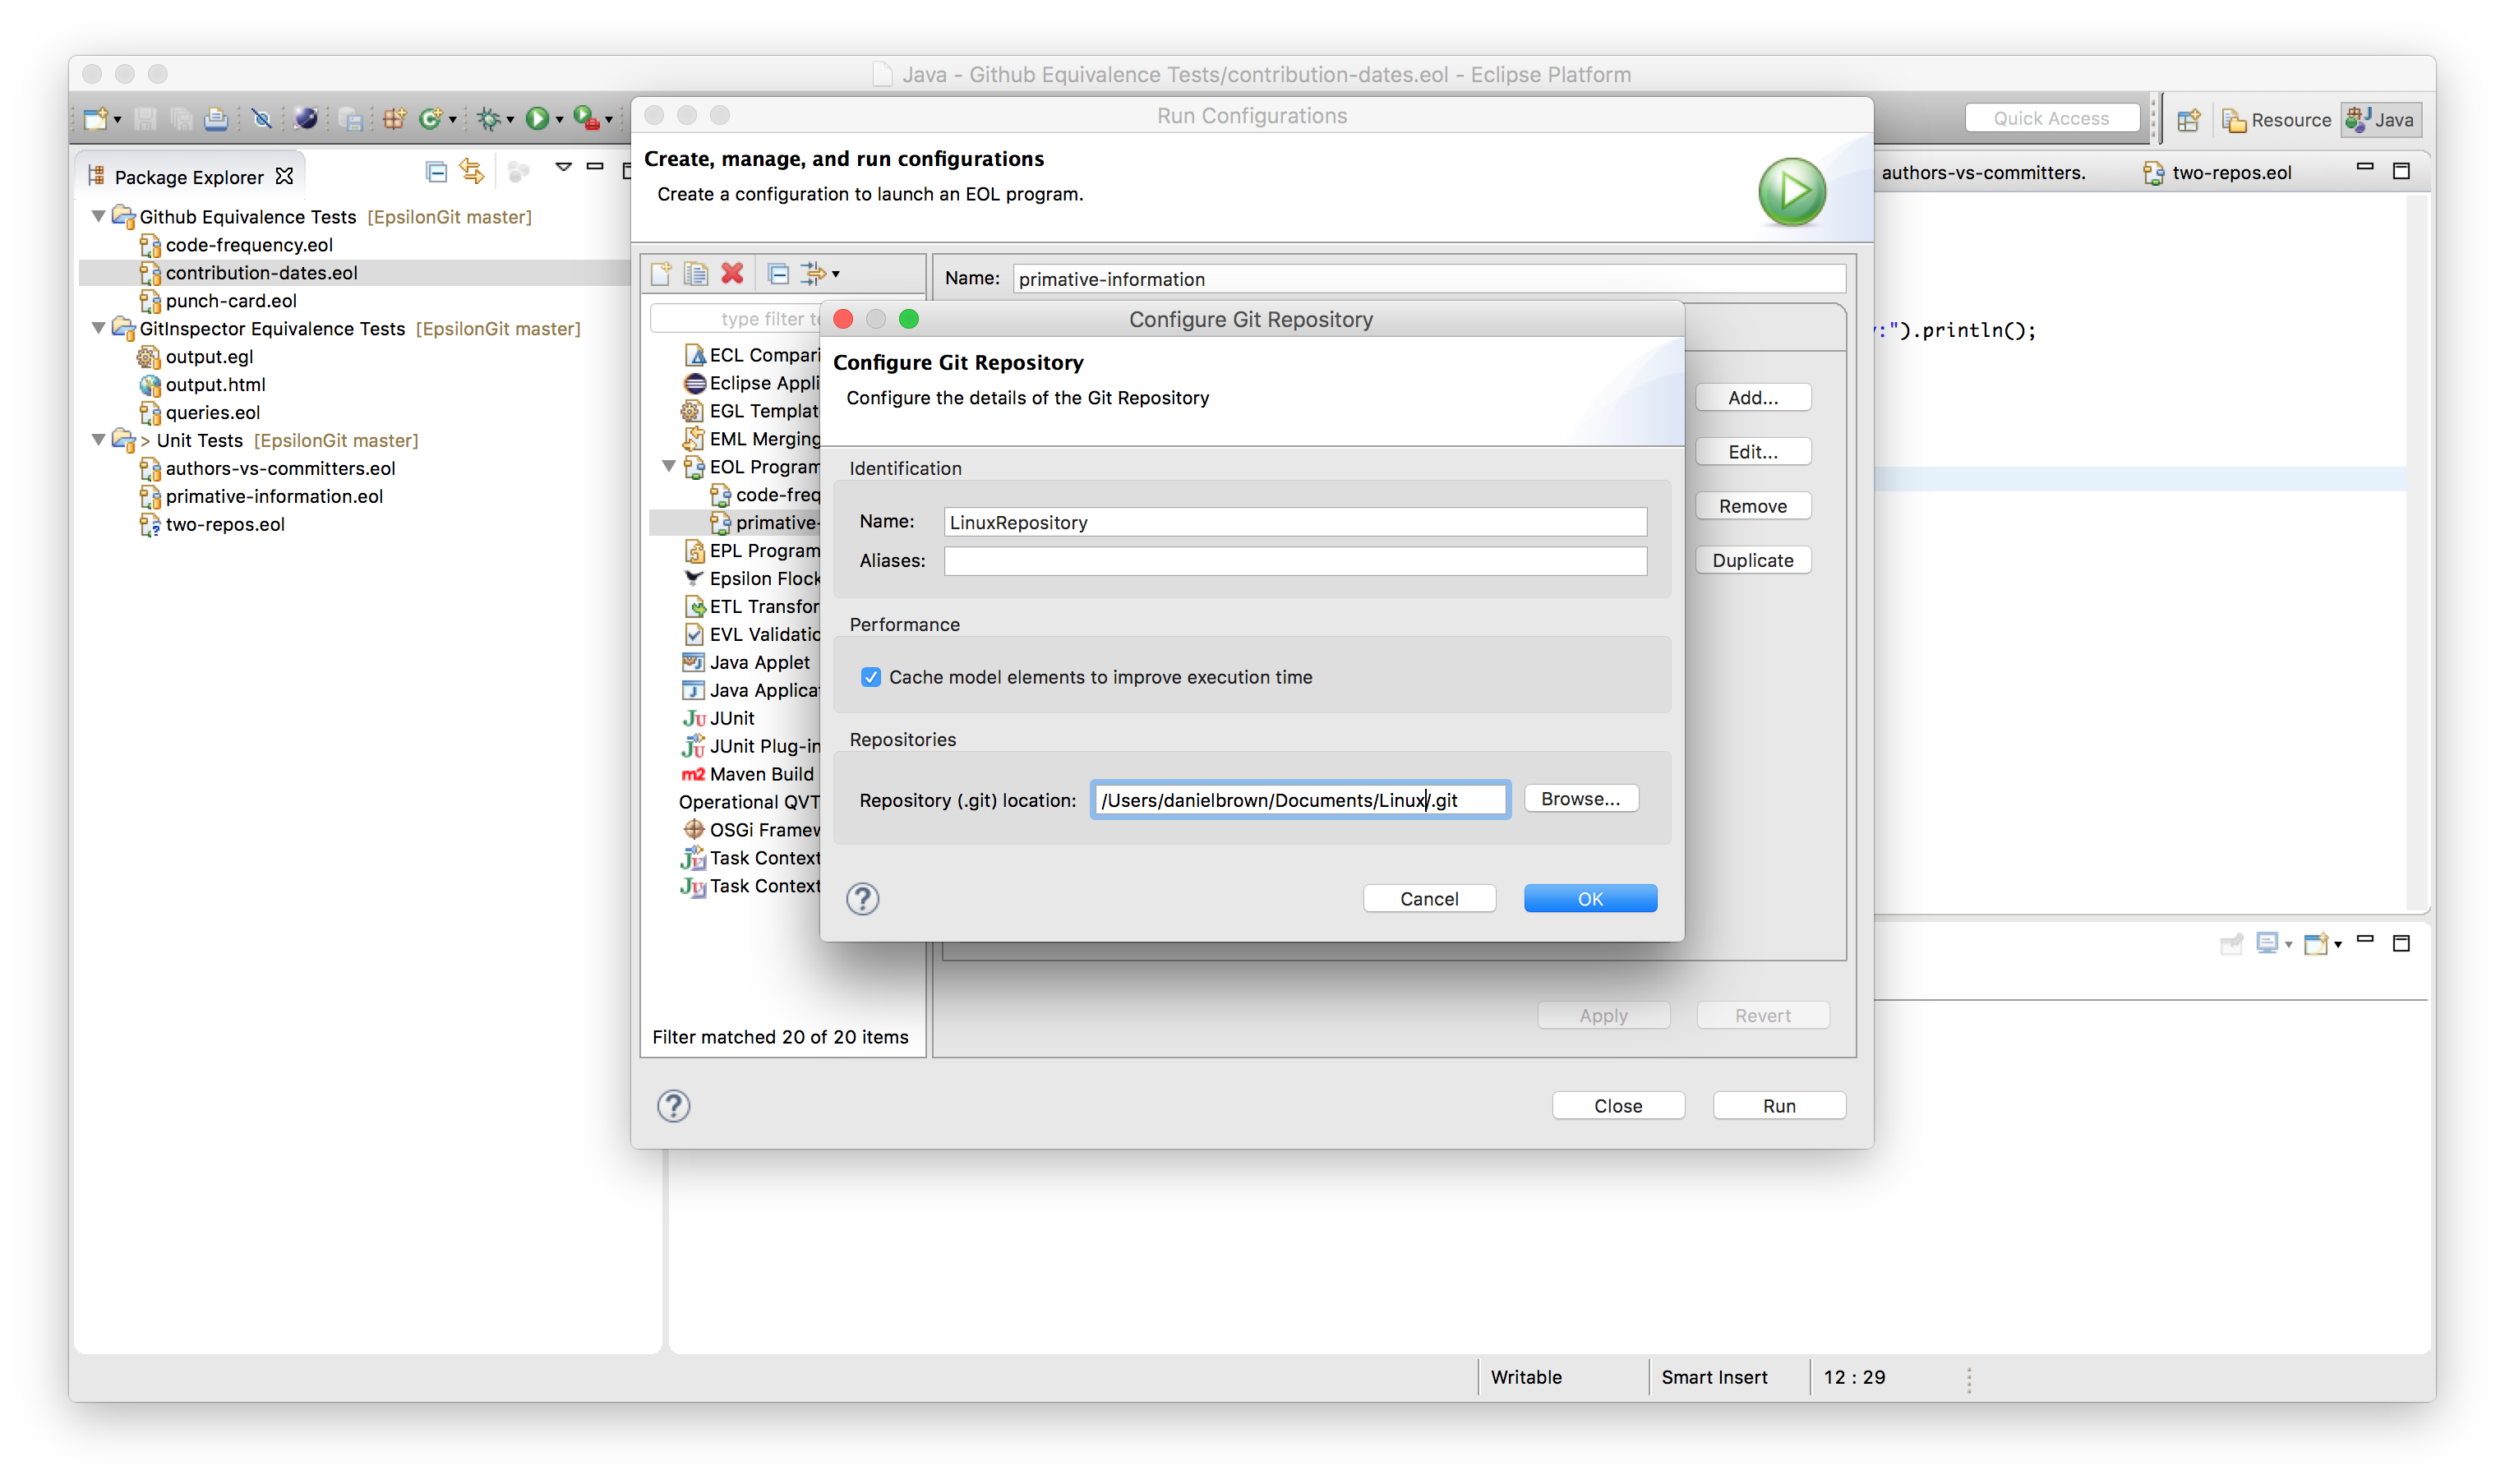
\includegraphics[width=\textwidth]{images/epsilonintegration}
	\caption{EpsilonGit configuration dialog}
	\label{fig:epsilonintegration}
\end{figure}

SY-F-3 requires that a GUI consistent with the rest of the epsilon suite be accessible for users to add git models for querying and analysis to Epsilon -- this too can be seen being satisfied in Figure \ref{fig:epsilonintegration}. Due to the fact that this configuration dialog allows a user to enter the location of their git repository and therefore EOL code doesn't need to have this hardcoded EpsilonGit also satisfies requirement SH-F-4, "Query Developers should be able to develop epsilon object language code which requires no knowledge of the underlying git repository and can therefore be distributed for others to know about"

\section{Acceptance Tests}
\label{evalacceptance}
Whilst the unit tests proved that the code written did what was expected of it, it did nothing to ensure that the software developed actually met the initial specification and project requirements.

Acceptance tests specify the desired behaviour of the system and are a type of formal testing conducted to determine whether or not a system satisfies its acceptance criteria and to enable the customer to determine whether or not to accept the system \cite{acceptancetests1}\cite{acceptancetests2}. 

Acceptance tests for EpsilonGit consisted of a set of Epsilon Object Language scripts, which should execute successfully with an acceptable solution, written prior to development of production code. 

The acceptance tests presented as Listings A.1-A.5 were written to prove that read access to all the most common parts of git was available through Epsilons domain specific languages and generators, satisfying requirements SH-F-1, SH-F-3, SH-F-1 and SY-F-2. Acceptance test A.6 compares the amount of commits in two repositories and outputs a message saying which has more -- thus proving EpsilonGit satisfies requirement SH-F-2, "Git Analysts should be able to access multiple git repositories at once for comparison".

Each of these tests can be executed using Epsilon and EpsilonGit and provide results consistent with those provided by the competing solutions -- therefore all EOL acceptance tests passed.

\section{Comparison with Existing Solutions}
Sections \ref{evalepsilonintegration} and \ref{evalacceptance} outline how EpsilonGit has met both its stakeholder and system functional requirements. However, they do not prove that the solution produced for this project has met or exceeded its non-functional requirements relating to speed or ease-of-use compared to the existing solutions detailed in section \ref{competitors}.

In this section performance and ease-of-development relating to bespoke queries will be compared with GitInspector, GitHub and Gitana.

\subsection{Performance}
Each of the tools being compared here is rather different, each using different programming languages and libraries, which can make comparing performance difficult. After much consideration the author has decided that performance will be measured in the amount of time required to perform a specified query. CPU and memory usage will not be measured.

Some of the systems may fair better with repositories of different sizes, so a small repository, medium sized repository and large repository will be used for evaluation. The small repository is for one of the authors side projects, called csblogs, and consists of 411 commits \cite{csbrepository}. The medium sized repository is for the node.js runtime and consists of 10,762 commits \cite{noderepository}. The large repository is the linux kernel repository, which consists of 535,010 commits \cite{linuxrepository}.

 

%TODO : Eval

\subsection{Ease of Query Development}
Code complexity is itself a complex topic. There are several ways to measure complexity including cyclomatic complexity and halstead volumes \cite{halstead}. However, it was decided that a simpler metric of lines of code to produce a pre-determined result would be easier to analyse and sufficient to determine if the ease-of-use requirements had be satisfied.

%TODO : Eval

\section{Overall Review}
Allowing access to git, a software repository, via a model-driven interface is both a novel and powerful application of Model Driven Engineering that will allow both the author and other software engineers to write queries useful for analysing git repositories in order to uncover interesting and actionable information about software systems.

The integration with the epsilon platform both makes the use of epsilon more attractive to software engineers in general and allows existing modelling engineers to query git repositories with the same ease as they can any other Epsilon Model Connectivity format.

The author intends to submit a paper to both to MSR 2016 -- The 13th Working Conference on Mining Software Repositories \cite{msr2016} -- and a future International Conference on Model Driven Engineering Languages and Systems.

% Explain use of TDD, both unit tests, integration and use of EOL files that it would be hoped would work with
% Automated testing
% Use of CI
% Testing against requirements
% Summary (did all test pass?)
% Does it at least fulfil all of the analysis and querying required by the two systems its competing with (github and gitinspector?)
% Case Study vs GitInspector
	% Comparison of lines of code and code complexity required for the same output
	% Comparison of Run Time on same hardware

\chapter{Conclusion}
% Project Review (Chronological rundown of what happened)
\section{Project Review}
This project set out with the task of bringing easy to develop, customisable and bespoke queries to git repositories by using model-driven engineering techniques. 

The project started by conducting a thorough review of the literature concerning version control systems, git, the internals and uses of the git system, existing tools to analyse git repositories and model driven engineering -- particularly using Epsilon.

A problem statement was written outlining the problem to be solved, which allowed the author to identify stakeholders in the process and use the information about their use cases to determine the exact requirements of the project.

The requirements of the project and the likelihood of change present in any research project suggested to the author that he should be using an agile methodology -- a mixture of Scrum, Kanban and Extreme Programming was adopted to suite the exact requirements and constraints of the project.

Design and implementation took place iteratively, and allowed for experimentation. Once the features outlined in the requirements phase of the project were complete the system was evaluated against its competitors.

\section{Project Success}
Overall this project has been a success. The system envisioned at the beginning of the process has been delivered, as proven by the acceptance tests outlined in chapter \ref{testeval}.

Model-Driven Engineering has proven itself to be a highly effective way of dealing with complex structured data -- both in terms of reducing query complexity and enabling more bespoke and complex queries -- and the author thinks that model-driven engineerings role in mining software repositories should be further researched.

If the project were to be done over again then the author would do little differently -- many design and implementation issues were fixed through the use of the iterative methodology -- however he would have written more acceptance tests covering more of Epsilons domain specific languages \& generators and written more helper methods for some of the object model elements.

The author is personally very excited to see what novel analysis can be made on git repositories by third-parties using the EpsilonGit software.

The success of this project could be built upon in future by implementing or researching some of ideas presented in section \ref{potentialfuturework}.

\section{Potential Future Work}
\label{potentialfuturework}
% Currently read only, would be interesting to see if being able to author commits etc via epsilon could be useful. Or even the ability to change names on commits etc via http://stacktoheap.com/blog/2013/01/06/using-mailmap-to-fix-authors-list-in-git/
% Make it would with subversion, mercurial etc
% Transform from git to svn/mercurial or vice versa via ETL (lots of people would want to make this transition)
% Lots of low hanging fruit regarding performance (e.g. computing properties each time instead of storing them in memory once they've been worked out once)
Whilst the current design and implementation of EpsilonGit matches the requirements set out for this project it would be possible for a future project to build on the work completed for this one to improve EpsilonGit in a number of ways. 

In Chapter \ref{design} it is discussed how the system provides read only access to git repositories. If the project was continued it would be possible to add write access via the domain specific languages provided by Epsilon. This could allow the following functionality:

\begin{enumerate}
	\item Authoring of commit messages
	\item Deletion of commits by using the \code{git reset} command \cite{gitreset}
	\item Managing of merging and branching
	\item Retrospectively changing the name or contact details of authors and committers in the system using git mailmap \cite{gitmailmap}
\end{enumerate} 

It is unknown if there would be benefit to a user in having a model driven interface for making changes to a git repository -- this too could be researched. 

A larger addition to EpsilonGit could be to make it compatible with other popular version control systems -- such as Mercurial and Apache Subversion. Adding in compatibility with these systems, alongside write support, would enable the use of EpsilonGit to migrate from one version control system to another, as well as providing the analysis and querying functionality presented in this report for git.

Chapter \ref{design} discusses some of the design decisions made, such as the use of caching, to improve the performance of the EpsilonGit system. However, due to the size of the project and the time constraints imposed upon it there are some low hanging fruit regards performance improvement. For example, whilst the model elements themselves are cached, some of the results of methods ran on them are not -- e.g. every time \code{commit.getCommitCalendar()} is called a new calendar object is initialised -- these could be cached for future use.

The secondary aim of this project is the increase the interest amongst developers in Epsilon and Model Driven Engineering. The project, as is, is required to be used through Epsilon Eclipse, which includes many useful model driven engineering tools, but may be too large a piece of software to download, install and manage for someone who just wants to analyse one software repository -- putting people off of using EpsilonGit and therefore not finding out more about MDE. This could be resolved in future by allowing a developer to download a program which just includes EpsilonGit, a texteditor to write epsilons domain specific languages, and the required Epsilon Libraries, or by providing them with an online interface to these features.

At the time of writing a fellow student is developing a web accessible system for generating artefacts from and querying models and structured artefacts that are accessible using Epsilon Model Connectivity. The ability to query analyse git through a web interface could be useful and so it would be interesting to consider combining the two systems in future.

\section{Reflection}
In this section the author will reflect on the project as a whole and his ability to deliver it both on time and to the initial specification.

% TDD was great, agile working seemed to work well.
Overall it is felt that the project went reasonably well, especially as all of the initial aims and objectives were met. The methodology used, in particular the test-driven development aspects, were well suited to the project and made developing a solution to a complicated problem simpler in the long-run -- though did of course require some up-front time investment.

% Java code is pretty reasonable, took a little while to get into but previous C# knowledge helped
It is felt that the quality of the code produced for the project was quite high and could certainly be reused or extended in the future if need be -- perhaps with some ideas from section \ref{potentialfuturework}. There was a very slight learning curve for the author as he comes from a background of primarily C\# development. Whilst C\# and Java are fairly similar as languages -- both garbage collected, object-oriented and with a syntax inspired by C -- their standard libraries are rather different. The author in particular remembers having to use the \code{Apache.Commons.Lang} library to use some features which come out-of-the-box in C\#, like \code{NotImplementedException}s.

% Example EOL/EGX code works well, but might be better if more declarative 
The EOL code used as acceptance tests for the solution is also felt to be of good quality -- in the respects that it is easily readable and can be explained easily -- however the author acknowledges that less lines of code would have been required had it been written in a more declarative style rather than imperative. 

% Working on project whilst other 'real life' stuff happens
% Working on coming back to a project after a long time 
In section \ref{constaints} the main constraint of this project was identified as time. This was certainly true, but to a higher degree than was expected. During the period of time in which the project was scheduled to run the author had to find employment for after his studies and find somewhere close to that employment to live -- both of these activities took longer than the author naively assumed they would. This extended period of time devoted to house and job hunting led to a second problem, having to re-learn the project after an extended period of time away from it -- fortunately good note taking and good commit messages in version control stopped this from being a big issue. 

% This is one of only a few large projects I've worked on, so it was good experience
EpsilonGit has been a rather large project, in terms of the number of technologies involved, the number of lines of code itself and the amount of literature review required to be able to design something novel in the field. The author is sure that the experience of developing a project of this magnitude will aid him in his future endevours.

\printbibliography

\begin{appendices}
\noappendicestocpagenum
\addappheadtotoc
\chapter{EOL Acceptance Test Code}
\label{eolacceptance}

\begin{lstlisting}[caption=Punchcard, label=lst:punchcard]
var currentDay;
var commitsInHour : Map;
for(commit in Commit.all.sortBy(c | c.getCommitCalendar().getDayOfWeekValue())) {
	var commitCalendar = commit.getCommitCalendar();
	var commitDay = commitCalendar.getDayOfWeek();
	if(not (commitDay == currentDay)) {
		if(not(currentDay == null)) {
			//This commit occured in the next type of day. Print out current days info.
			currentDay.println();
			commitsInHour.println();
			"".println();
		}
		
		//Reset
		currentDay = commitDay;
		commitsInHour.clear();
	}
	
	//Get hour of commit and add to list
	var hourOfCommit = commitCalendar.getHours();
	if(commitsInHour.containsKey(hourOfCommit)) {
		commitsInHour.put(hourOfCommit, commitsInHour.get(hourOfCommit) + 1);
	}
	else {
		commitsInHour.put(hourOfCommit, 1);
	}
}
\end{lstlisting}
\clearpage
\begin{lstlisting}[caption=Contribution Dates, label=lst:contributiondates]
"The following number of commits happened per day across the whole repository:".println();
printDatesToCommits(Commit.all);
"\n\n".print();

for(committer in Committer.all) {
	(committer.getName() + " (" + committer.getEmailAddress() + ") committed this many times per day:").println();
	printDatesToCommits(committer.getAllCommittedCommits());
	"\n\n".print();
}

operation printDatesToCommits(commitsList) {  
	var datesToNumberCommits : Map;
	for(commit in commitsList.sortBy(c | c.getCommitCalendarDate())) {
		var commitDate = commit.getCommitCalendarDate();
	
		if(datesToNumberCommits.containsKey(commitDate)) {
			datesToNumberCommits.put(commitDate, datesToNumberCommits.get(commitDate) + 1);
		}
		else {
			datesToNumberCommits.put(commitDate, 1);
		}
	}
	
	for(date in datesToNumberCommits.keySet().sortBy(k | k)) {
		(date.getDay() + "/" + date.getMonth() + "/" + date.getYear()).print();
		" - ".print();
		datesToNumberCommits.get(date).print();
		" commits".println();
	}
}
\end{lstlisting}
\clearpage
\begin{lstlisting}[caption=Commit frequency, label=lst:commitfrequency]
"Week".format("%-30s | ").print();
"Commits".format("%-13s | ").print();
"Insertions".format("%-13s | ").print();
"Deletions".format("%-13s | ").println();
"--------------------------------------------------------------------------------".println();


var startOfWeek;
var endOfWeek;
var numberCommits = 0;
var numberAdditions = 0;
var numberRemovals = 0;

for(commit in Commit.all.reject(c | c.isMergeCommit()).sortBy(c | c.getCommitCalendarDate())) {
	
	var commitDate = commit.getCommitCalendarDate();
	
	if(endOfWeek == null) {
		//This is the first commit. Lets set up our weeks...
		//Week start on a Sunday. We grab the sunday before this first commit. (this is how Github works! madness!)
		startOfWeek = commitDate.getPreviousDay("Sunday");
					
		endOfWeek = startOfWeek.addDays(6);
	}
	
	while(commitDate.compareTo(endOfWeek) > 0) {
		//This commit belongs in a later week...
		//First print current week data
		(formatDate(startOfWeek) + " - " + formatDate(endOfWeek)).format("%-30s | ").print();

		numberCommits.format("%-13s | ").print();
		numberAdditions.format("%-13s | ").print();
		numberRemovals.format("%-13s | ").println();
		
		//Iterate to next week
		startOfWeek = endOfWeek.addDays(1);
		endOfWeek = startOfWeek.addDays(6);	
		
		//Reset counts
		numberCommits = 0;
		numberAdditions = 0;
		numberRemovals = 0;
	}
	
	// Add to this weeks totals
	var differenceCount = commit.getDifferenceCountFromParent();
	numberCommits = numberCommits + 1;	
	numberAdditions += differenceCount.getLinesAdded();
	numberRemovals += differenceCount.getLinesRemoved();
}

operation formatDate(date) {
	return (date.getDay() + "/" + date.getMonth() + "/" + date.getYear());
}
\end{lstlisting}

\begin{lstlisting}[caption=GitInspector-style output, label=lst:gitinspectorequivilence]
"The following historical commit information, by author, was found in this repository:\n".println();
"Author".format("%-60s | ").print();
"Commits".format("%-13s | ").print();
"Insertions".format("%-13s | ").print();
"Deletions".format("%-13s | ").print();
"% of Changes".format("%-13s |").println();
"---------------------------------------------".println();

//Work out totals
var totalRepositoryAdditions : Real;
var totalRepositoryRemovals : Real;
for(commit in Commit.all.reject(a | a.isMergeCommit())) {
	var differenceCounts = commit.getDifferenceCountFromParent();
	totalRepositoryAdditions += differenceCounts.getLinesAdded();
	totalRepositoryRemovals += differenceCounts.getLinesRemoved();
}
var totalRepositoryChanges : Real = totalRepositoryAdditions + totalRepositoryRemovals;
	
for(author in Author.all.sortBy(a | a.getName())) {
	(author.getName() +" (" + author.getEmailAddress() + ")").format("%-60s | ").print();	
	author.getAllAuthoredCommits().size().asInteger().format("%-13d | ").print();
	
	var commitsByAuthor = author.getAllAuthoredCommits().reject(a | a.isMergeCommit());
		
	var totalAuthorInsertions : Real;
	var totalAuthorDeletions : Real;
	for(commit in commitsByAuthor) {
		var differenceCounts = commit.getDifferenceCountFromParent();
		totalAuthorInsertions += differenceCounts.getLinesAdded();
		totalAuthorDeletions += differenceCounts.getLinesRemoved();
	}
	var totalAuthorChanges : Real = totalAuthorInsertions + totalAuthorDeletions;
	
	totalAuthorInsertions.asInteger().format("%-13d | ").print();
	
	totalAuthorDeletions.asInteger().format("%-13d | ").print();
	
	if(totalAuthorChanges == 0) {
		"0%".format("%-13s |").println();
	}
	else {
		(((totalAuthorChanges / totalRepositoryChanges) * 100).format("%.2f") + "%").format("%-13s |").println();
	}
}
\end{lstlisting}

\begin{lstlisting}[caption=Author vs Committer Information, label=lst:authorvscommitter]
var onlyAuthors = Author.all.excludingAll(Committer.all).sortBy(a | a.getName());
if(onlyAuthors.size() > 0) {
	("The following " + onlyAuthors.size() + " authors are not committers: ").println();
	for(author in onlyAuthors) {
		("* " + author.getName() + " (" + author.getEmailAddress() + ")").println();
	} 
}
else {
	"All authors are also comitters".println();
}

"".println();
"------".println();
"".println();

var onlyCommitters = Committer.all.excludingAll(Author.all).sortBy(a | a.getName());
if(onlyCommitters.size() > 0) {
	("The following " + onlyCommitters.size() + " committers are not authors: ").println();
	for(committer in onlyCommitters) {
		("* " + committer.getName() + " (" + committer.getEmailAddress() + ")").println();
	}
}
else {
	"All committers are also authors".println();
}
\end{lstlisting}
\clearpage
\begin{lstlisting}[caption=Author vs Committer Information, label=lst:multirepos]
var repoOneSize = RepoOne!Commit.all.size();
var repoTwoSize = RepoTwo!Commit.all.size();
if(repoOneSize == repoTwoSize) {
	"Repositories have same number of commits".println();
}
else
{
	if(repoOneSize > repoTwoSize) {
		"Repository one has more commits".println();
	}
	else {
		"Repository two has more commits".println();
	}
}
\end{lstlisting}

\end{appendices}

\end{document}
